\chapter{强化学习的心理学} \label{chap:chap11}

在前面的章节中,我们仅基于计算考虑就提出了算法的想法。
在本章中,我们从另一个角度来看其中的一些算法:心理学的角度及其对动物如何学习的研究。
本章的目的是,首先,讨论强化学习的思想和算法与心理学家对动物学习的发现相对应的方式,其次,解释强化学习对动物学习研究的影响。
事实证明,强化学习提供的清晰形式主义将任务,回报和算法系统化,在理解实验数据,提出新的实验种类以及指出可能对操作和测量至关重要的因素方面非常有用。
长期优化回报的想法是强化学习的核心,这有助于我们理解动物学习和行为的其他令人困惑的特征。


强化学习与心理学理论之间的一些对应关系并不令人惊讶,因为强化学习的发展受到了心理学学习理论的启发。
然而,正如本书所述,强化学习从人工智能研究人员或工程师的角度探索理想化的情况,目的是用有效的算法解决计算问题,而不是复制或详细解释动物如何学习。
因此,我们描述的一些通信将各自领域中独立产生的想法联系起来。
我们认为这些接触点特别有意义,因为它们揭示了对学习很重要的计算原理,无论是通过人工还是通过自然系统学习。


在大多数情况下,我们描述了强化学习和学习理论之间的对应关系,这些理论是为了解释大鼠,鸽子和兔子等动物如何在受控实验室实验中学习而开发的。
在整个20世纪进行了数千次这样的实验,其中许多至今仍在进行中。
虽然有时被认为与心理学中更广泛的问题无关,但这些实验探索了动物学习的微妙特性,通常是由精确的理论问题驱动的。
随着心理学将重点转移到行为的更多认知方面,即思维和推理等心理过程,动物学习实验在心理学中的作用比以前少了。
但是,这项实验导致了学习原则的发现,这些原则在整个动物界都是基本的和广泛的,这些原则在设计人工学习系统时不应该被忽视。
此外,正如我们将看到的那样,认知处理的某些方面自然地与强化学习提供的计算视角相关联。


本章的最后一节包括与我们讨论的联系以及我们忽视的联系相关的参考文献。
我们希望本章鼓励读者更深入地探讨所有这些联系。
最后一节还讨论了强化学习中使用的术语与心理学术语的关系。
强化学习中使用的许多术语和短语都是从动物学习理论中借用的,但是这些术语和短语的计算/工程意义并不总是与其在心理学中的意义一致。


\section{预测和控制}


我们在本书中描述的算法分为两大类:预测算法和控制算法。
这些类别自然出现在强化学习问题的解决方法中。
在许多方面,这些类别分别对应于心理学家广泛研究的学习类别:经典或巴甫洛夫式条件作用和工具性或操作性条件作用。
由于心理学对强化学习的影响,这些对应关系并不完全是偶然的,但它们仍然引人注目,因为它们将来自不同目标的想法联系起来。


本书中介绍的预测算法估计的数量取决于代理环境的特征在未来的发展情况。
我们特别关注于估计代理在与环境交互时未来可能获得的回报量。
在这个角色中,预测算法是策略评估算法,它是改进策略算法的组成部分。
但预测算法不仅限于预测未来的回报;他们可以预测环境的任何特征\cite{modayil2014prediction}。
预测算法和经典条件反射之间的对应关系取决于它们预测即将到来的刺激的共同特性,无论这些刺激是否有益(或惩罚)。


仪器或操作条件实验的情况是不同的。
在这里,实验装置的设置是为了根据动物的行为给予动物喜欢的东西(奖励)或不喜欢的东西(惩罚)。
动物学会增加产生奖励行为的倾向,减少产生惩罚行为的倾向。
据说强化刺激取决于动物的行为,而在经典条件反射中则不然(尽管在经典条件反射实验中很难消除所有行为偶然性)。
仪器调节实验就像我们在第一章中简要讨论的那些启发\textit{桑代克}效应定律的实验。
控制是这种学习形式的核心,它对应于强化学习的策略改进算法的操作。


在预测方面思考经典条件反射,在控制方面思考工具条件反射,是将我们的强化学习的计算观点与动物学习联系起来的起点,但实际上,情况比这更复杂。
经典条件作用比预测更多;它还涉及行动,控制模式也是如此,有时被称为巴甫洛夫控制。
此外,经典和工具性条件反射以有趣的方式相互作用,这两种学习都可能在大多数实验情况下进行。
尽管存在这些复杂性,但将经典/工具区别与预测/控制区别相结合是将强化学习与动物学习联系起来的方便的rst近似。


在心理学中,强化一词用于描述经典条件反射和工具条件反射的学习。
最初只指强化一种行为模式,也经常用于弱化一种行为模式。
被认为是行为改变原因的刺激被称为增强剂,它是否取决于动物以前的行为。
在本章的末尾,我们将更详细地讨论这个术语,以及它与机器学习中使用的术语的关系。


\section{经典条件反射} \label{sec:classical_conditioning}

在研究消化系统的活动时,著名的俄罗斯生理学家\textit{伊万$\cdot$巴甫洛夫}发现,动物对某些触发刺激的先天反应可能会被与先天触发因素无关的其他刺激触发。
他的实验对象是经过小手术的狗,以准确测量其唾液re-ex的强度。
在他描述的一个案例中,这只狗在大多数情况下都不会流涎,但在喂食后约5秒钟,它会在接下来的几秒钟内产生约6滴唾液。
在几次重复呈现另一种刺激后,一种与食物无关的刺激,在这种情况下是节拍器的声音,在引入食物之前不久,狗对节拍器的声音做出了唾液分泌的反应,就像它对食物的反应一样。
“因此,唾液腺的活动被声音的冲动所激发,这是一种与食物完全不同的刺激”。
巴甫洛夫总结了这一发现的重要性,写道:


很明显,在自然条件下,正常动物不仅必须对自身带来直接好处或伤害的刺激作出反应,而且还必须对其他物理或化学机构(声波,光波等)作出反应,这些物理或化学机构本身只发出这些刺激的接近信号;
虽然猎物的视觉和声音本身对较小的动物有害,但它的牙齿和爪子有害。


以这种方式将新刺激与先天性反应联系起来,现在被称为经典或巴甫洛夫条件反射。
\textit{巴甫洛夫}将先天性反应(例如,上述演示中的流涎)称为\textit{非条件反射},其自然触发刺激(例如食物)\textit{非条件刺激},以及由预测刺激触发的新反应(例如,这里还有流涎)\textit{条件反射}。
最初是中性的刺激,意味着它通常不会引起强烈的反应(例如节拍器声音),当动物知道它预测\textit{非条件刺激}并因此产生\textit{条件反射}以响应\textit{条件刺激}时,它就会成为\textit{条件刺激}。
这些术语仍然用于描述经典的条件反射实验(尽管更好的翻译应该是“有条件的”和“无条件的”,而不是有条件的和无条件的)。
\textit{非条件刺激}被称为强化者,因为它强化了对\textit{条件刺激}产生\textit{条件反射}的反应。


右侧显示了两种常见类型的经典调节实验中刺激的排列。
在延迟调节中,\textit{条件刺激}延伸到整个刺激间隔或\textit{刺激间距},这是\textit{条件刺激}发作和\textit{非条件刺激}发作之间的时间间隔(当\textit{非条件刺激}以此处显示的常见版本结束时,\textit{条件刺激}结束)。
在跟踪条件反射中,\textit{非条件刺激}在\textit{条件刺激}结束后开始,\textit{条件刺激}o集合和\textit{非条件刺激}开始之间的时间间隔称为跟踪间隔。


\begin{figure}[!htb]
	\centering
	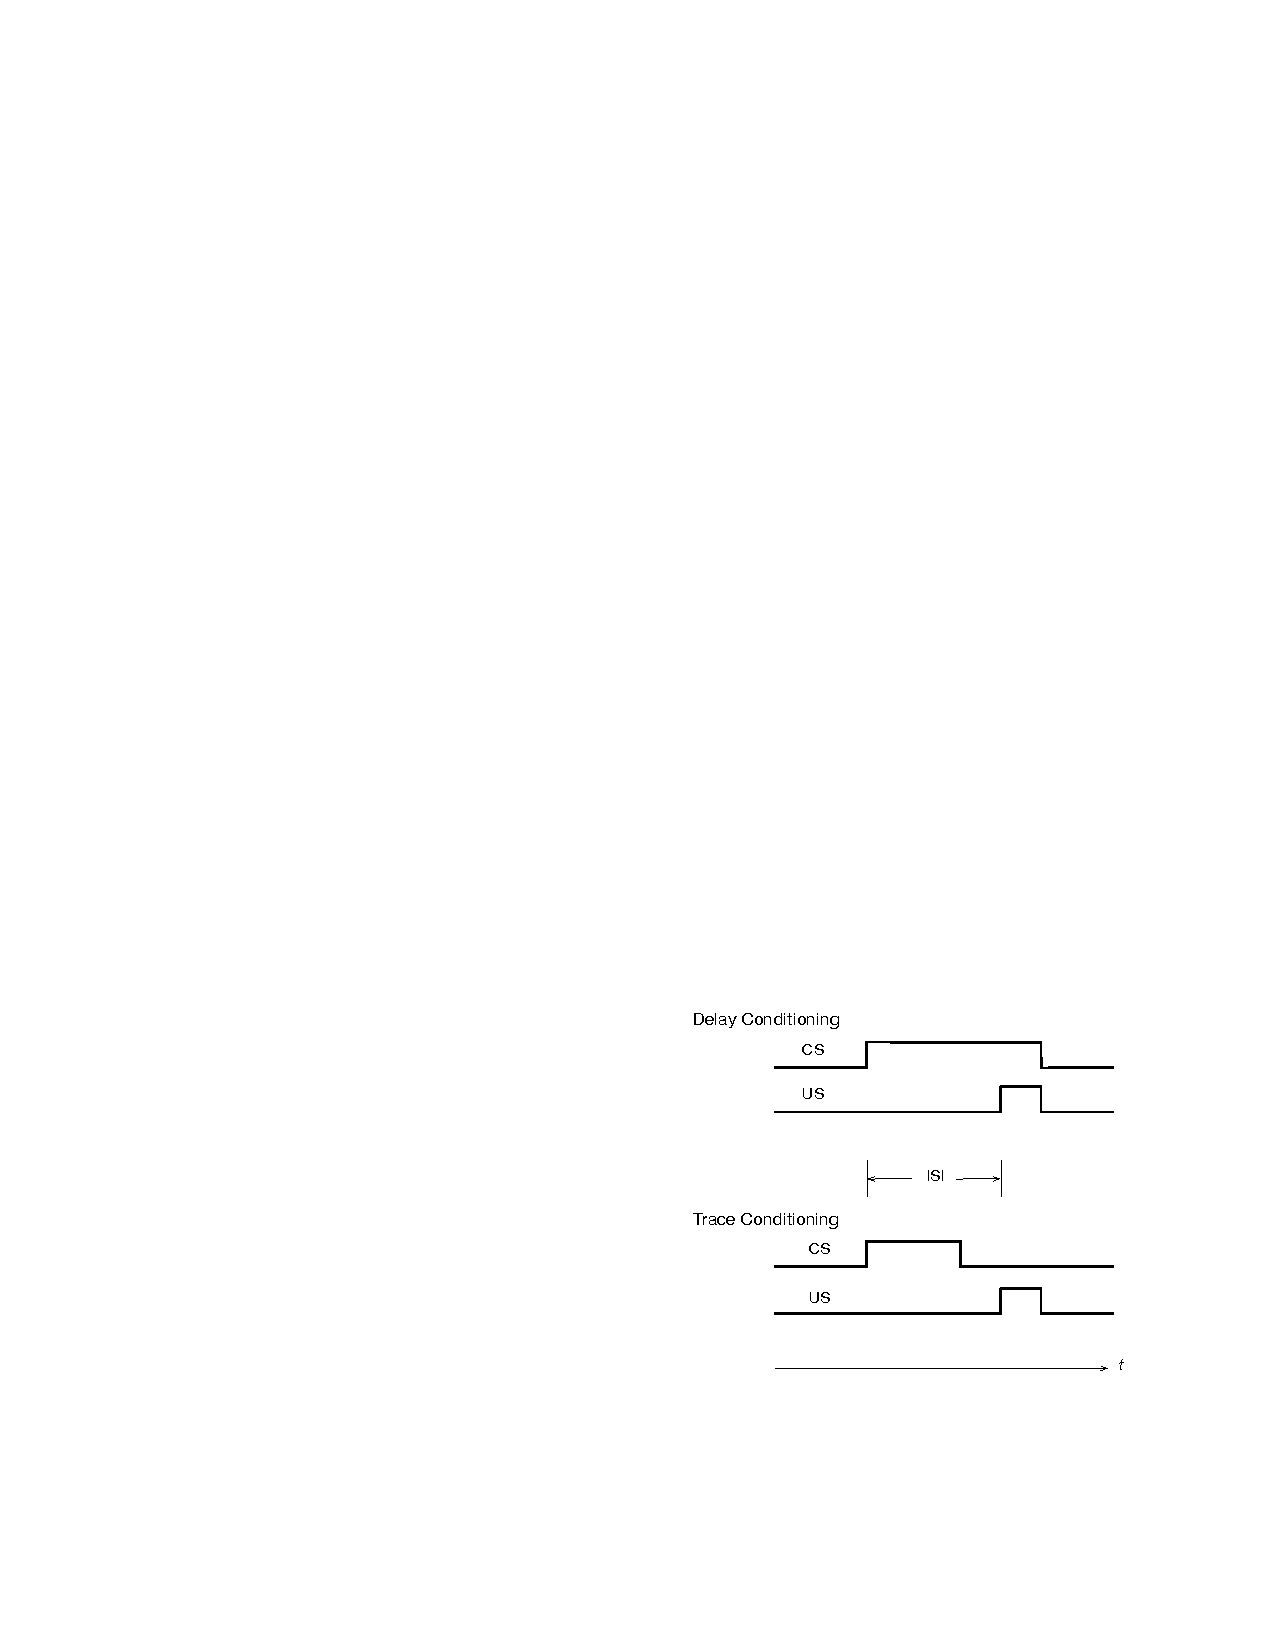
\includegraphics[width=0.5\linewidth]{chap11/fig_11_0}
	\caption{  \label{fig:11_0}}
\end{figure}


巴甫洛夫的狗对节拍器的声音流涎只是经典条件反射的一个例子,已经在许多动物的许多反应系统中进行了深入研究。
\textit{非条件反射}通常在某种程度上是准备性的,比如巴甫洛夫的狗流涎,或者在某种程度上是保护性的,比如对刺激眼睛的东西眨眼,或者看到捕食者时冻结。
在一系列试验中经历\textit{条件刺激}-\textit{非条件刺激}预测关系会使动物了解到\textit{条件刺激}预测\textit{非条件刺激},因此动物可以通过\textit{条件反射}对\textit{条件刺激}做出反应,为动物做好准备或保护其免受预测的\textit{非条件刺激}的影响。
一些\textit{条件反射}类似于\textit{非条件反射},但开始得更早,并且以增加其有效性的方式开始。
例如,在一项深入研究的实验中,音调\textit{条件刺激}可靠地预测了兔子眼睛的空气(\textit{非条件刺激}),触发了\textit{非条件反射},该\textit{非条件反射}由称为切口膜的保护性内眼睑闭合组成。
在一次或多次试验后,音调开始触发由膜闭合组成的\textit{条件反射},该膜闭合在吹空气之前开始并最终定时,以便在吹空气可能发生时发生峰值闭合。
这种\textit{条件反射}是在预期吹空气和适当时间的情况下启动的,比简单地启动关闭作为对刺激我们的反应更好。
通过学习刺激之间的预测关系来预测重要事件的能力是如此有益,它广泛存在于动物界。





\subsection{阻塞和高阶条件反射} \label{sec:blocking_higher_order}

在实验中已经观察到经典条件反射的许多有趣性质。
除了\textit{条件反射}的预期性质之外,在经典调节模型的发展中,两个广泛观察到的特性得到了显着体现:阻塞和高阶调节。
当一个潜在的\textit{条件刺激}与之前用于调节动物产生\textit{条件反射}的另一个\textit{条件刺激}一起出现时,当动物无法学习\textit{条件反射}时,就会发生阻塞。
例如,在涉及兔子切口膜调节的阻断实验的第一阶段,兔子首先用音调\textit{条件刺激}和吹空气 \textit{非条件刺激}调节,以产生在预期吹空气的情况下关闭其切口膜的\textit{条件反射}。
实验的第二阶段包括额外的试验,其中第二个刺激(例如光)被添加到音调中以形成复合音调/光\textit{条件刺激},然后是相同的吹空气 \textit{非条件刺激}。
在实验的第三阶段,仅第二个刺激(即光)被呈现给兔子,以查看兔子是否已经学会了用\textit{条件反射}对其作出反应。
结果表明,兔子对光的反应产生了很少或没有\textit{条件反射}:对光的学习已经被先前对音调的学习所阻止。
这样的阻止结果挑战了这样的观点,即调节只依赖于简单的时间连续性,即必要和足够的条件条件反射是\textit{非条件刺激}经常在时间上紧跟\textit{条件刺激}。
在下一节中,我们将描述\textit{雷斯科拉-瓦格纳模型}\cite{rescorla1972theory},该模型为阻塞提供了全面的解释。
	


当先前条件化的\textit{条件刺激}充当\textit{非条件刺激}来调节另一个最初中性的刺激时,就会发生高阶条件化。
如上所述,巴甫洛夫描述了一个实验,在这个实验中,他的助手首先调节一只狗,让它随着节拍器的声音流涎,节拍器可以预测食物的味道。
在这个调节阶段之后,进行了许多试验,其中将狗最初独立的黑色方块放置在狗的视线中,然后是节拍器的声音,而不是食物。
在仅仅十次试验中,这只狗只在看到黑色方块时才开始流涎,尽管事实上,看到它之后从来没有食物。
节拍器的声音本身就像一个\textit{非条件刺激},将流涎的\textit{条件反射}调节为黑色方块\textit{条件刺激}。
这是二阶条件反射。如果黑色方块被用作\textit{非条件刺激}来建立另一个中性\textit{条件刺激}的唾液\textit{条件反射},那么它将是三阶条件反射,等等。高阶条件反射很难证明,特别是在二阶以上,部分原因是高阶增强剂由于在高阶条件反射试验中没有被原\textit{非条件刺激}反复遵循而失去了增强价值。
但是在正确的条件下,例如将一阶试验与高阶试验混合或通过提供一般的激励刺激,可以证明二阶以上的高阶条件反射。
正如我们在下面所描述的,经典条件反射的\textit{时间差分}模型使用了自举思想,这是我们的方法的核心,以扩展\textit{雷斯科拉-瓦格纳模型}对阻塞的描述,以包括\textit{条件反射}的预期性质和高阶条件反射。
	
	
高阶仪器调节也会发生。
在这种情况下,持续预测初级强化的刺激本身就变成了强化剂,如果通过进化将其奖励或惩罚的品质建立在动物体内,则强化是主要的。
预测刺激成为二级增强剂,或者更一般地说,是高阶或条件性增强剂--当预测的增强刺激本身是二级或甚至更高阶的增强剂时,后者是更好的术语。
条件性强化剂提供条件性强化:条件性奖励或条件性惩罚。
条件性强化就像初级强化一样,增加动物产生导致条件性奖励的行为的倾向,并减少动物产生导致条件性惩罚的行为的倾向。
(请参阅本章末尾的评论,解释我们的术语有时与心理学中使用的术语有何不同。)



条件性强化是一个关键现象,它解释了为什么我们为条件性强化货币工作,而条件性强化货币的价值完全来自于拥有它所预测的东西。
在第13.5节描述的\textit{行动者}-\textit{评论家}方法(并在第15.7节和第15.8节的神经科学背景下进行了讨论)中,\textit{评论家}使用\textit{时间差分}方法来评估\textit{行动者}的政策,其价值估计为\textit{行动者}提供了条件性强化,从而使\textit{行动者}能够改进其政策。
这种更高阶的工具性条件作用的类似物有助于解决第1.7节中提到的信贷分配问题,因为当主要奖励信号延迟时,评论家会对\textit{行动者}进行瞬间强化。
我们将在下面的第14节中对此进行更多讨论。四。


\subsection{雷斯科拉-瓦格纳模型} \label{sec:rescorla_wagner}

\textit{雷斯科拉}和\textit{瓦格纳}创建模型主要是为了解释阻塞。
\textit{雷斯科拉-瓦格纳模型}的核心思想是,动物只有在事件违反其预期时才能学习,换句话说,只有当动物感到惊讶时(尽管不一定意味着任何有意识的期望或情绪)。
我们首先使用\textit{雷斯科拉}和\textit{瓦格纳}的术语和符号来呈现模型,然后再转向我们用来描述\textit{时间差分}模型的术语和符号。


以下是\textit{雷斯科拉}和\textit{瓦格纳}如何描述他们的模型。
该模型调整化合物\textit{条件刺激}的每个成分刺激的“关联强度”,这是一个数字,表示该成分预测\textit{非条件刺激}的强度或可靠性。
当在经典调节试验中呈现由多个成分刺激组成的化合物\textit{条件刺激}时,每个成分刺激的关联强度的变化方式取决于与整个刺激化合物相关的关联强度,称为“聚合关联强度”,而不仅仅取决于每个成分本身的关联强度。


\textit{雷斯科拉}和\textit{瓦格纳}考虑了一种化合物\textit{条件刺激} AX,由成分刺激A和X组成,其中动物可能已经经历了刺激A,而刺激X可能是动物新的。设$V_A$,$V_X$和$V_{AX}$分别表示刺激A,X和化合物AX的结合强度。
假设在试验中,化合物\textit{条件刺激} AX后面跟着一个\textit{非条件刺激},我们将其标记为刺激Y。
然后刺激成分的关联强度根据以下表达式变化:

\begin{equation}
	\Delta V_A = \alpha_A \beta_Y
		(R_Y - V_{AX})
\end{equation}


\begin{equation}
	\Delta V_X = 
		\alpha_X \beta_Y
		(R_Y - V_{AX})
\end{equation}

其中A Y和X Y是步长参数,取决于\textit{条件刺激}分量和\textit{非条件刺激}的恒等式,Y是\textit{非条件刺激} Y可以支持的结合强度的渐近水平。
(\textit{雷斯科拉}和\textit{瓦格纳}在这里使用R代替R,但我们使用R是为了避免与我们使用and混淆,因为我们通常认为这是奖励信号的大小,但需要注意的是,经典条件反射中的\textit{非条件刺激}不一定是奖励或惩罚的。)该模型的一个关键假设是总联想强度VAX等于VA+VX。
由这些s改变的关联强度在下一次试验开始时成为关联强度。


为了完成,该模型需要一种响应生成机制,这是一种将V s值映射到\textit{条件反射}的方法。
因为这种映射将取决于实验情况的细节,所以\textit{雷斯科拉}和\textit{瓦格纳}没有指定映射,而是简单地假设较大的V s会产生更强或更可能的\textit{条件反射},并且负V s意味着不会有\textit{条件反射}。


\textit{雷斯科拉-瓦格纳模型}以一种解释阻塞的方式解释了\textit{条件反射}的获取。
只要刺激化合物的总结合强度VAX低于\textit{非条件刺激}Y可以支持的结合强度RY的渐近水平,预测误差RY􀀀VAX为正。
这意味着在连续的试验中,成分刺激的关联强度VA和VX增加,直到总关联强度VAX等于RY,此时关联强度停止变化(除非\textit{非条件刺激}改变)。当将新组分添加到动物已经调理过的化合物\textit{条件刺激}中时,用增强化合物进一步调理会使添加的\textit{条件刺激}组分的缔合强度几乎没有增加,或者没有增加,因为误差已经减小到零或低值。
\textit{非条件刺激}的发生几乎已经被完美地预测到了,因此新的\textit{条件刺激}组件几乎没有引入错误或惊喜。先前的学习阻碍了对新组件的学习。


为了从\textit{雷斯科拉}和\textit{瓦格纳}的模型过渡到经典条件反射的\textit{时间差分}模型(我们称之为\textit{时间差分}模型),我们根据本书中使用的概念重新构建了他们的模型。
具体来说,我们将用于学习的符号与线性函数近似(第9.4节)相匹配,并且我们认为调节过程是在试验中基于该试验中提出的化合物\textit{条件刺激}“学习预测\textit{非条件刺激}的大小”的过程之一,其中\textit{非条件刺激}Y的大小是如上所述的\textit{雷斯科拉-瓦格纳模型}的Y。
我们还引入了状态。因为\textit{雷斯科拉-瓦格纳模型}是一个试验级模型,这意味着它处理了从试验到试验的联想强度如何变化,而不考虑试验内部和试验之间发生的任何细节,我们不必考虑在试验期间状态如何变化,直到我们在下一节。
相反,在这里,我们简单地将状态视为根据试验中存在的组件\textit{条件刺激}的集合来标记试验的一种方式。


因此,假设试验类型或状态s由特征x(s)=(x1(s)的实值向量描述;x2(s);:::;xd(s))>如果试验中存在化合物\textit{条件刺激}的第i个组分CSi,则xi(s)=1,否则为0。
然后,如果结合强度的d维向量为w,则试验类型s的总结合强度为

\begin{equation}\label{key}
	v(s, \textbf{w}) = 
		w^T x(s).
\end{equation}
这对应于强化学习中的价值估计,我们认为它是\textit{非条件刺激}的预测。

现在暂时让t表示完整试验的次数,而不是它作为时间步长的通常含义(当我们将其扩展到下面的\textit{时间差分}模型时,我们恢复到t的通常含义),并假设St是对应于试验t的状态。
调节试验t将关联强度向量wt更新为wt+1,如下所示:

\begin{equation}\label{key}
	w_{t+1} = w_t + \alpha \delta_t x(S_t),
\end{equation}

步长参数在哪里,因为这里我们描述的是\textit{雷斯科拉-瓦格纳模型}| t是预测误差
	
\begin{equation}\label{key}
	\delta = R_t - v (S_t, w_t).
\end{equation}


Rt是试验t预测的目标,即\textit{非条件刺激}的规模,或者用\textit{雷斯科拉}和\textit{瓦格纳}的话说,是\textit{非条件刺激}在试验中可以支持的联合强度。
请注意,由于(14.2)中的因子x(St),因此只有试验中存在的\textit{条件刺激}组件的关联强度才能作为该试验的结果进行调整。
你可以将预测误差视为惊喜的衡量标准,将总联想强度视为动物的期望,当它与\textit{非条件刺激}的目标幅度不匹配时,就会被违反。


从机器学习的角度来看,\textit{雷斯科拉-瓦格纳模型}是一种纠错监督学习规则。它本质上与最小均方(LMS)或Widrow-Ho学习规则(Widrow and Ho,1960)相同,该规则将权重(这里是关联强度),使所有误差的平方平均值尽可能接近零。
它是一种“曲线”或回归算法,广泛用于工程和科学应用(见第9.4节)。3


\textit{雷斯科拉-瓦格纳模型}在动物学习理论的历史上是非常重要的,因为它表明一个“机械”理论可以解释关于阻塞的主要事实,而不需要诉诸更复杂的认知理论,例如,动物明确认识到另一个刺激成分已被添加,然后向后扫描其短期记忆,以重新评估涉及\textit{非条件刺激}的预测关系。
\textit{雷斯科拉-瓦格纳模型}显示了传统的连续性调节理论,即刺激的时间连续性是学习的必要和充分条件,可以通过一种简单的方式来调整,以解释阻塞(Moore和Schmajuk,2002年)2008年)。
	
	
\textit{雷斯科拉-瓦格纳模型}提供了经典条件反射的阻塞和其他一些特征的简单说明,但它不是经典条件反射的完整或完美模型。
不同的想法解释了各种其他观察到的影响,并且在理解经典条件反射的许多微妙之处方面仍在取得进展。
我们接下来描述的\textit{时间差分}模型虽然也不是经典条件反射的完整或完美模型,但它扩展了\textit{雷斯科拉-瓦格纳模型},以解决刺激之间的试验内和试验间的时间关系如何影响学习以及如何产生更高阶的条件反射。
	

\subsection{时间差分}

\textit{时间差分}模型是一个实时模型,而不是像\textit{雷斯科拉-瓦格纳模型}这样的试验级模型。在我们上面的\textit{雷斯科拉-瓦格纳模型}的公式中,一个单步t代表了一个完整的条件反射试验。
该模型不适用于关于试验期间发生的事情或试验之间可能发生的事情的细节。
在每个试验中,动物可能会经历各种刺激,这些刺激的发作发生在特定的时间,并且具有特定的持续时间。
这些时间关系强烈影响学习。
\textit{雷斯科拉-瓦格纳模型}也不包括高阶条件反射的机制,而对于\textit{时间差分}模型,高阶条件反射是\textit{时间差分}算法基础上的自举思想。
	
	
	
为了描述\textit{时间差分}模型,我们从上面的\textit{雷斯科拉-瓦格纳模型}的公式开始,但t现在标记了试验内或试验之间的时间步长,而不是完整的试验。将t和t+1之间的时间想象为一个小的时间间隔,例如0.01秒,并将试验视为一系列状态,每个时间步长都有一个关联,其中步骤t的状态现在表示刺激在t处如何表示的细节,而不仅仅是试验中\textit{条件刺激}成分的标签。
事实上,我们可以完全放弃试验的想法。
从动物的角度来看,试验只是其与世界相互作用的持续经验的一部分。
遵循我们通常的观点一个与环境相互作用的主体,想象动物正在经历一系列无尽的状态s,每个状态s都由特征向量x(s)表示。也就是说,将试验称为实验中刺激模式重复的时间片段仍然很方便。


状态特征不限于描述动物经历的外部刺激;它们可以描述外部刺激在动物大脑中产生的神经活动模式,这些模式可能与历史有关,这意味着它们可能是由外部刺激序列产生的持续模式。
当然,我们不确切知道这些神经活动模式是什么,但是像\textit{时间差分}模型这样的实时模型允许人们探索学习关于外部刺激的内部表征的不同假设的后果。
由于这些原因,\textit{时间差分}模型不适用于任何特定的状态表示。
此外,由于\textit{时间差分}模型包括跨越刺激之间时间间隔的折扣和资格痕迹,因此该模型还可以探索折扣和资格痕迹如何与刺激表征相互作用,以预测经典调节实验的结果。


下面我们描述了\textit{时间差分}模型中使用的一些状态表示及其含义,但目前我们对表示不可知,只假设每个状态s由特征向量x(s)=(x1(s)表示;x2(s);:::;xn(s))>。
然后(14.1)给出了对应于状态s的总结合强度,与\textit{雷斯科拉}-Wgner模型相同,但\textit{时间差分}模型不同地更新了结合强度向量w。
t现在标记了一个时间步长而不是一个完整的试验,\textit{时间差分}模型根据此更新来管理学习:

\begin{equation}\label{key}
	w_{t+1} = w_t + \alpha \delta_t z_t,
\end{equation}

它将\textit{雷斯科拉-瓦格纳模型}update(14.2)中的xt(St)替换为合格跟踪向量zt,而不是(14.3)的t,这里t是\textit{时间差分误差}:
	
	
\begin{equation}\label{key}
	\delta_t = 
		R_{t+1} + \gamma v (S_{t+1}, w_t) - v(S_t, w_t),
\end{equation}


其中是折扣因子(介于0和1之间),Rt是时间t的预测目标, v(St+1;wt)和 v(St;wt)是t+1和t的总结合强度,如(14.1)所定义的。


资格跟踪向量zt的每个分量i根据特征向量x(St)的分量xi(St)递增或递减,否则会以以下公式确定的速率衰减:

\begin{equation}\label{key}
	z_{t+1} = \gamma \lambda z_t 
		+ x(S_t).
\end{equation}

这是通常的资格跟踪衰减参数。

请注意,如果=0,\textit{时间差分}模型将简化为\textit{雷斯科拉-瓦格纳模型},但以下情况除外:t的含义在每种情况下都是不同的(\textit{雷斯科拉-瓦格纳模型}的试用号和\textit{时间差分}模型的时间步长),并且在\textit{时间差分}模型中,预测目标R中有一个时间步长领先。
\textit{时间差分}模型相当于具有线性函数近似的半梯度TD()算法的后视图(第12章),除了模型中的Rt不必像\textit{时间差分}算法用于学习用于政策改进的值函数时那样是奖励信号。



\subsection{时间差分模型仿真} \label{sec:td_simulation}

像\textit{时间差分}模型这样的实时调节模型很有趣,主要是因为它们可以预测试验级模型无法表示的各种情况。
这些情况涉及可调节刺激的时间和持续时间,这些刺激与\textit{非条件刺激}时间的关系,以及\textit{条件反射}的时间和形状。
例如,\textit{非条件刺激}通常必须在中性刺激开始后开始进行调节,学习的速度和有效性取决于\textit{刺激间距},即\textit{条件刺激}和\textit{非条件刺激}开始之间的间隔。
当\textit{条件反射}出现时,它们通常在\textit{非条件刺激}出现之前开始,并且在学习过程中其时间曲线发生变化。
在用复合\textit{条件刺激}调节时,复合\textit{条件刺激}的成分刺激可能不会同时开始和结束,有时会形成所谓的连续化合物,其中成分刺激会随着时间的推移以序列发生。
像这样的时间考虑因素使得重要的是要考虑刺激是如何表现的,这些表现如何在试验期间和试验之间随着时间的推移而展开,以及它们如何与折扣和资格痕迹相互作用。


图~\ref{fig:11_1}~显示了用于探索\textit{时间差分}模型行为的三种刺激表示:完整序列化合物(CSC),\textit{微刺激}和存在表示(Ludvig,Sutton和Kehoe,2012)。
这些表示在刺激存在的附近时间点之间强制泛化的程度不同。


\begin{figure}[!htb]
	\centering
	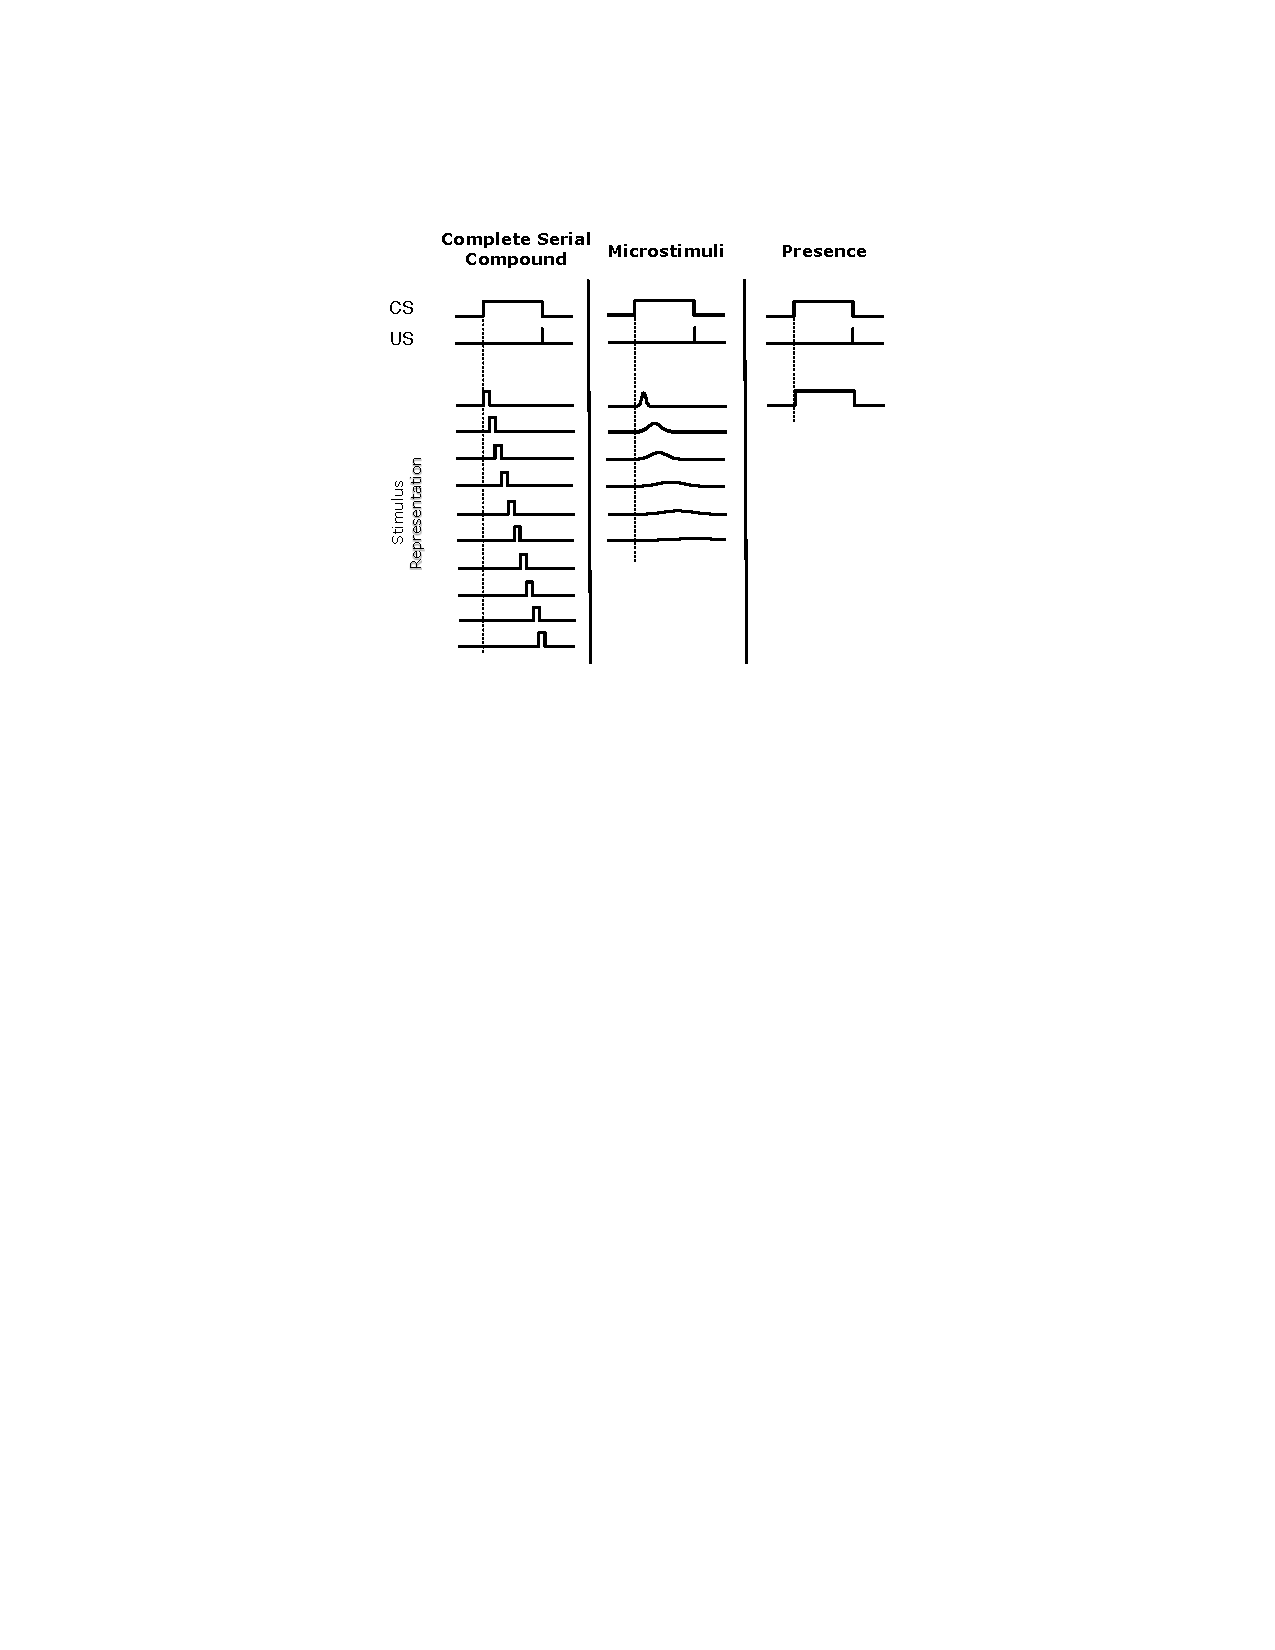
\includegraphics[width=0.5\linewidth]{chap11/fig_11_1}
	\caption{\textit{时间差分}模型有时使用三种刺激表示(列中)。
		每行代表刺激表示的一个元素。
		这三种表示沿时间泛化梯度变化,在完整序列化合物(左列)的附近时间点之间没有泛化,在存在表示(右列)的附近时间点之间没有完全泛化。
		微刺激表示占据了中间位置。时间泛化程度决定了学习\textit{非条件刺激}预测的时间粒度。
		改编自学习与行为的微小变化,《评估经典条件反射的TD模型》,第40卷,2012年,第311页,E.A.Ludvig,R.S.Sutton,E.J.Kehoe。经施普林格许可。  \label{fig:11_1}}
\end{figure}

图~\ref{fig:11_1}~所示的最简单表示是图右列中的存在表示。
这种表示对于试验中存在的每个成分\textit{条件刺激}都有一个单一的特征,每当该成分存在时,该特征的值为1,否则为0。
4存在表示并不是关于刺激如何在动物大脑中表示的现实假设,但正如我们下面描述的,具有这种表示的\textit{时间差分}模型可以产生经典条件反射中看到的许多时间现象。


对于CSC表示(图14.1的左栏),每个外部刺激的开始都会启动一系列精确定时的短期内部信号,直到外部刺激结束。
这就像假设动物的神经系统有一个时钟,在刺激呈现期间保持精确的时间轨迹;这就是工程师所说的分接延迟线。
“像存在表示一样,CSC表示作为大脑内部如何表示刺激的假设是不现实的,但Ludvig等人(2012)称之为有用的操作”,因为它可以揭示\textit{时间差分}模型在相对不受刺激表示约束时如何工作的细节。
CSC表示也用于大脑中产生多巴胺的神经元的大多数\textit{时间差分}模型中,这是我们在第15章中讨论的主题。
CSC表示通常被视为\textit{时间差分}模型的重要组成部分,尽管这种观点是错误的。


\textit{微刺激}表示(图~\ref{fig:11_1}~的中柱)类似于CSC表示,因为每个外部刺激都会引发一系列内部刺激,但在这种情况下,内部刺激(微刺激)并不是这种有限且不重叠的形式;
它们会随着时间的推移而延长并重叠。
随着刺激开始的时间流逝,不同的微刺激集变得或多或少活跃,并且随后的每个微刺激在时间上逐渐变宽并达到较低的最大水平。
当然,根据微刺激的性质,有许多\textit{微刺激}表征,文献中已经研究了许多\textit{微刺激}表征的例子,在某些情况下,还提出了动物大脑如何产生它们的建议(参见本章末尾的书目和历史评论)。
\textit{微刺激}表示比存在或CSC表示作为关于刺激的神经表示的假设更现实,并且它们允许\textit{时间差分}模型的行为与动物实验中观察到的更广泛的现象集合相关。
特别是,通过假设微刺激的级联是由\textit{非条件刺激}和\textit{条件刺激}发起的,并且通过研究微刺激,资格痕迹和折扣之间相互作用的学习的重要影响,\textit{时间差分}模型有助于构建假设来解释许多经典条件反射的微妙现象以及动物大脑如何产生它们。
下面我们将对此进行更多讨论,特别是在第15章中,我们将讨论强化学习和神经科学。


然而,即使有简单的存在表示,\textit{时间差分}模型也产生了\textit{雷斯科拉-瓦格纳模型}所解释的经典条件反射的所有基本特性,以及超出试验级模型范围的条件反射特征。
例如,正如我们已经提到的,经典条件反射的一个显着特征是,\textit{非条件刺激}通常必须在中性刺激开始后开始进行条件反射,并且在条件反射后,\textit{条件反射}在\textit{非条件刺激}出现之前开始。
换句话说,条件反射通常需要一个积极的\textit{刺激间距},\textit{条件反射}通常会预测\textit{非条件刺激}。
条件反射的强度(例如,\textit{条件刺激}引起的\textit{条件反射}的百分比)如何取决于不同物种和反应系统的\textit{刺激间距}差异很大,但它通常具有以下特性:对于零\textit{刺激间距}或负\textit{刺激间距},即当\textit{非条件刺激}发病与\textit{条件刺激}发病同时发生或早于\textit{条件刺激}发病时,它可以忽略不计(尽管研究发现关联强度有时会略有增加或与负\textit{刺激间距}呈负相关);
它在调节最有效的正\textit{刺激间距}处增加到最大值;
然后在响应系统变化很大的时间间隔后,它会减小到零。
\textit{时间差分}模型的这种依赖性的精确形状取决于其参数的值和刺激表示的细节,但\textit{刺激间距}依赖性的这些基本特征是\textit{时间差分}模型的核心属性。


串行复合条件反射产生的理论问题之一,即用成分按顺序出现的化合物\textit{条件刺激}进行条件反射,涉及促进远程关联。
已经发现,如果\textit{条件刺激}和\textit{非条件刺激}之间的空迹线间隔被第二个\textit{条件刺激}填充以形成连续的复合刺激,则有助于调节到第一个\textit{条件刺激}。
图~\ref{fig:11_2}~显示了\textit{时间差分}模型在这种实验的模拟中的行为,该实验的时间细节显示在图的顶部。与实验结果一致(Kehoe,1982),该模型显示由于存在第二个\textit{条件刺激},第一个\textit{条件刺激}的调节速率和渐近调节水平都得到了促进。

\begin{figure}[!htb]
	\centering
	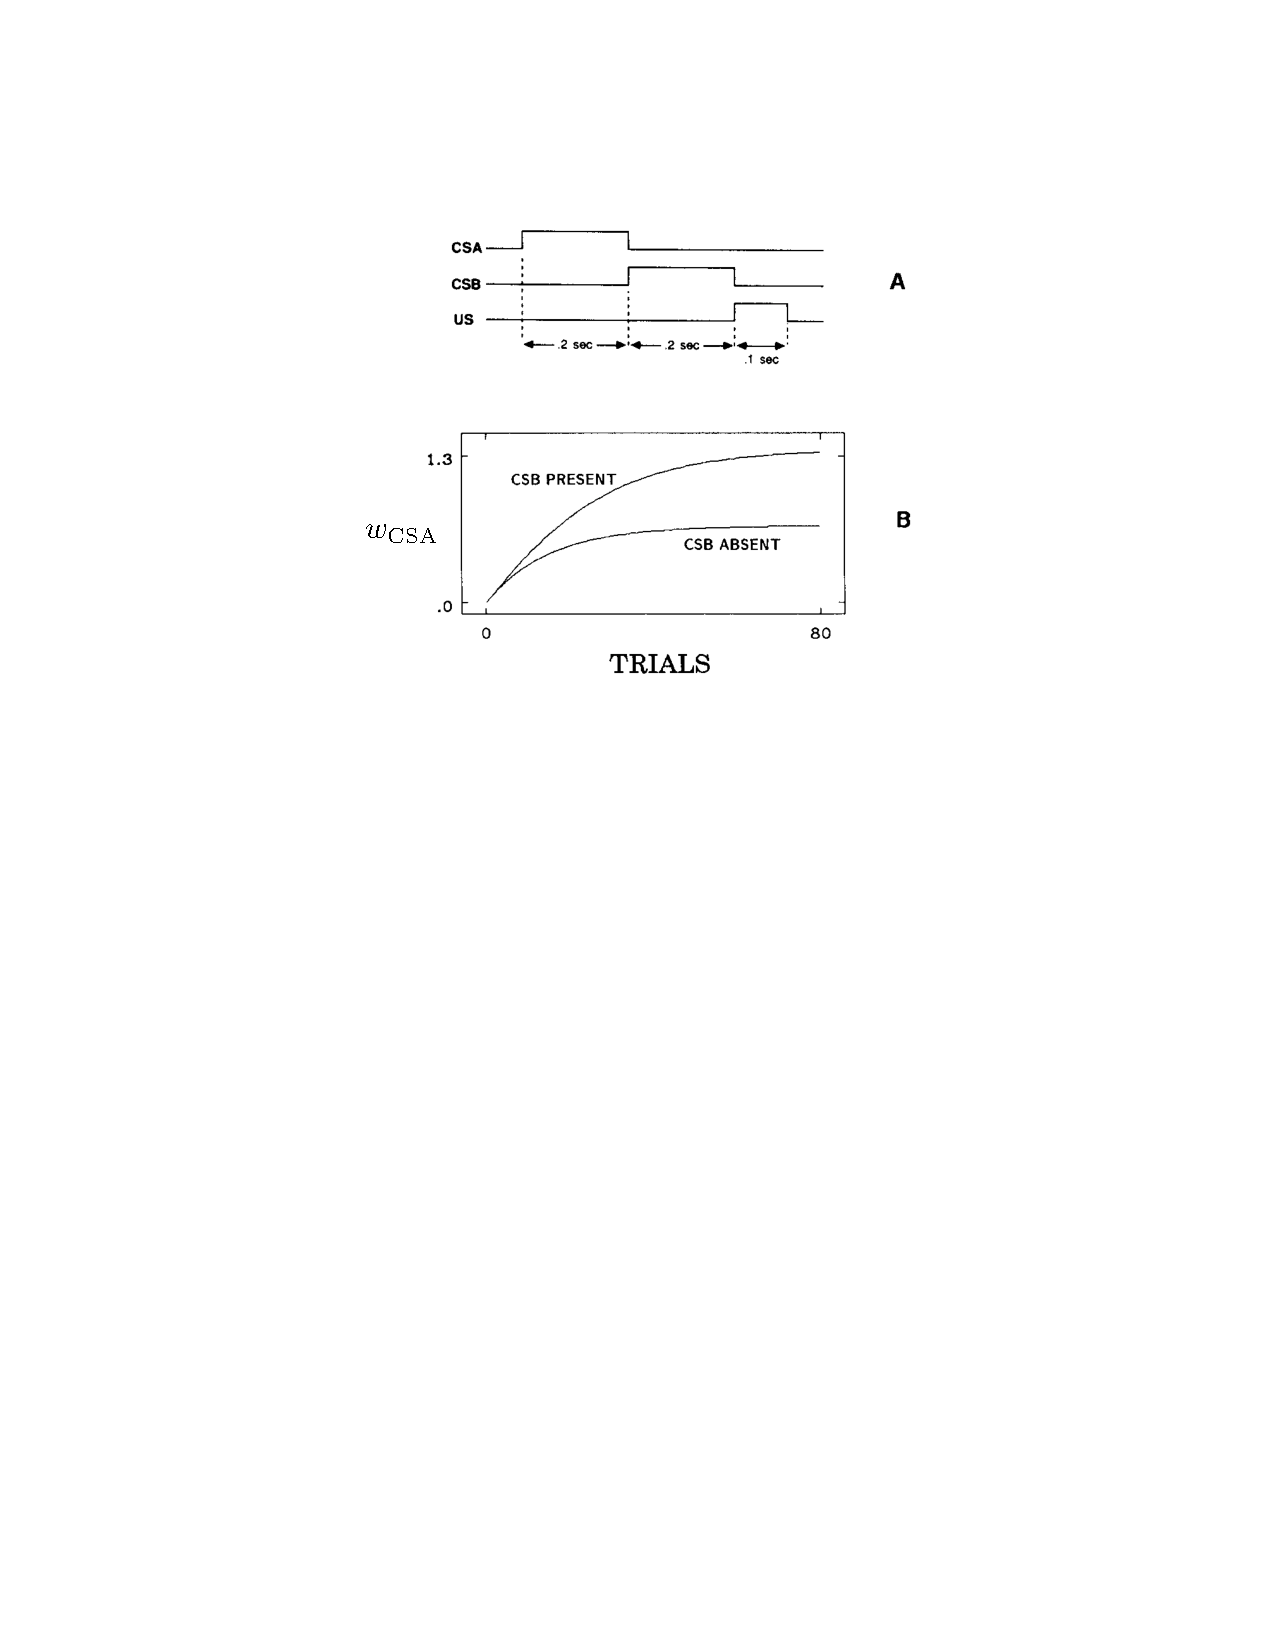
\includegraphics[width=0.5\linewidth]{chap11/fig_11_2}
	\caption{通过\textit{时间差分}模型中的干预刺激促进远程关联。
		上图:试验中刺激之间的时间关系。
		下图:当CSA以上图所示的连续化合物呈现时,以及当以与\textit{非条件刺激}相同的时间关系呈现时,仅在没有CSB的情况下,CSA的结合强度试验的行为。
		改编自Sutton和Barto(1990)。  \label{fig:11_2}}
\end{figure}


Egger和Miller(1962)的一项实验证明了试验中刺激之间时间关系的调节作用,该实验涉及延迟配置中的两个重叠\textit{条件刺激},如图~\ref{fig:11_3}~顶部所示。
尽管CSB与\textit{非条件刺激}的时间关系更好,但与不存在CSA的对照组相比,CSA的存在大大减少了对CSB的调节。
图~\ref{fig:11_3}~的底部面板显示了\textit{时间差分}模型在使用存在表示的实验模拟中产生的相同结果。

\begin{figure}[!htb]
	\centering
	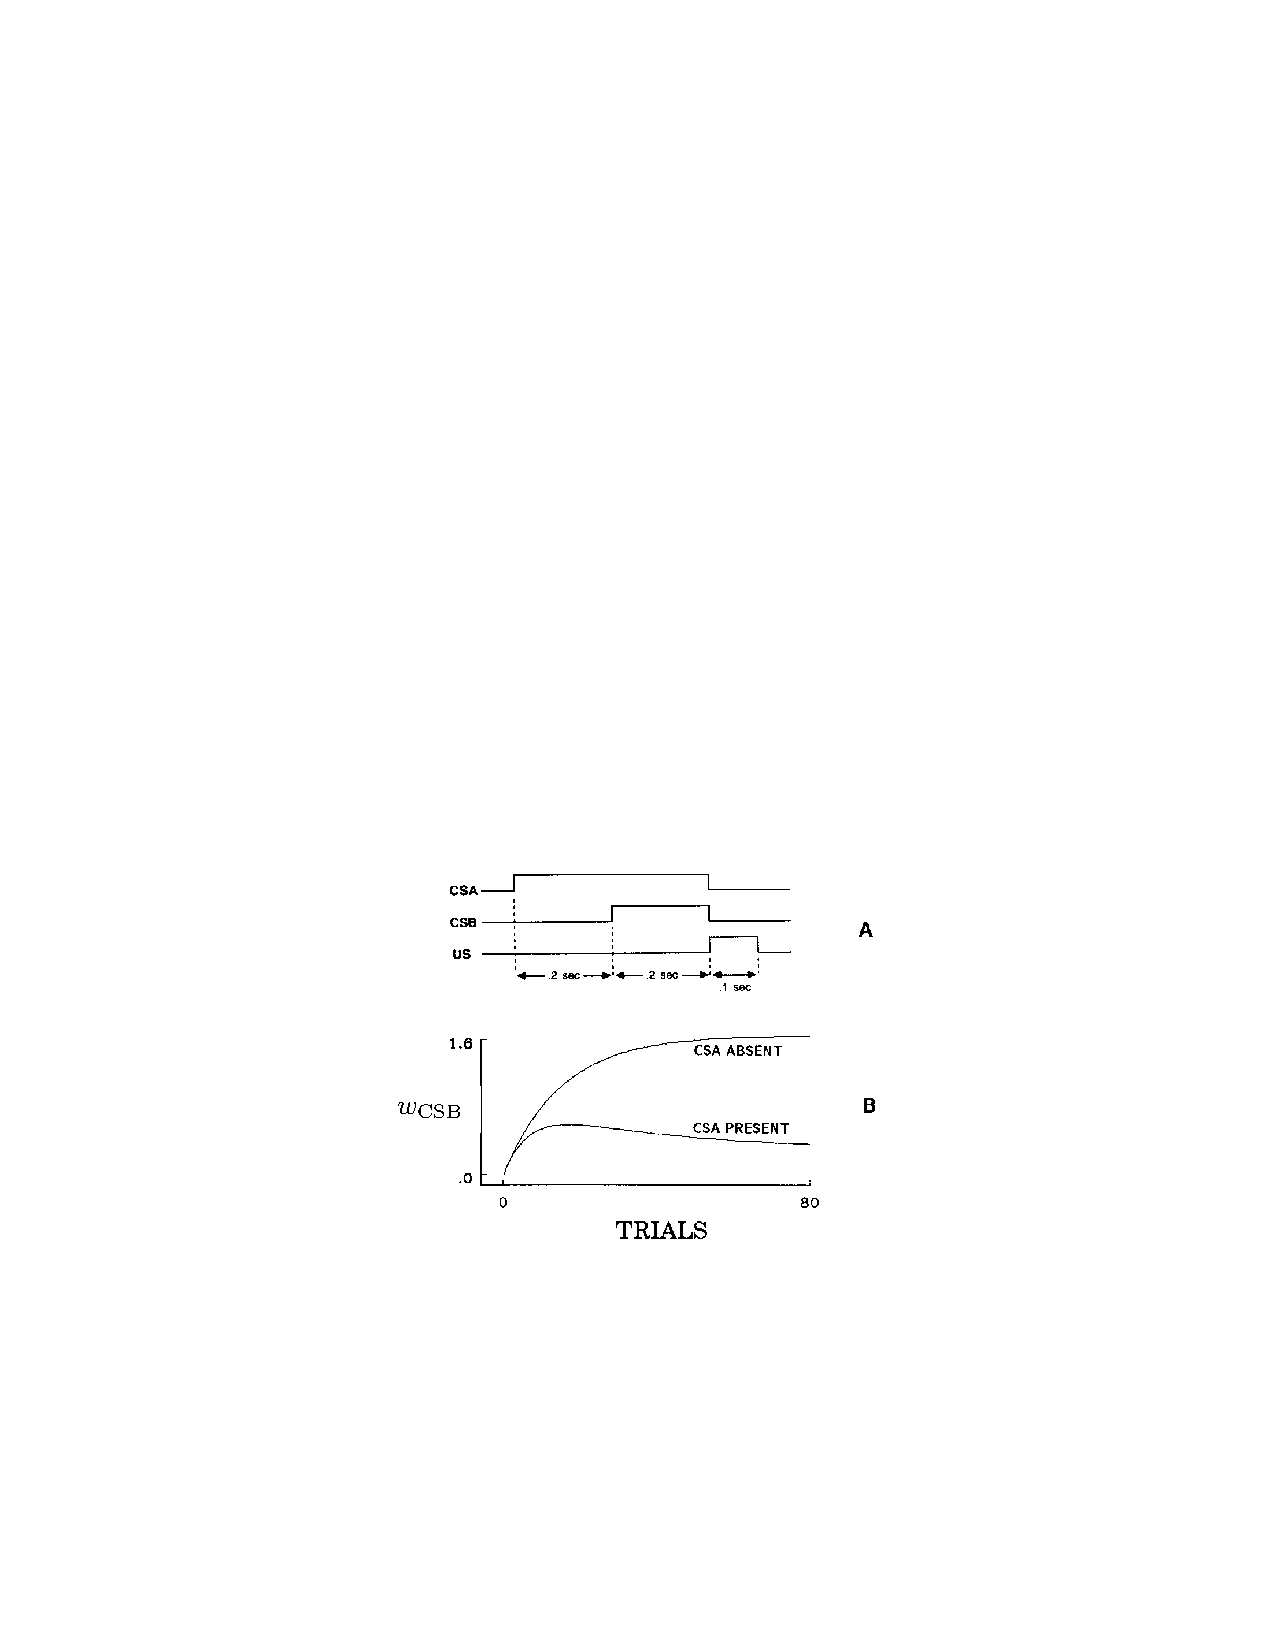
\includegraphics[width=0.5\linewidth]{chap11/fig_11_3}
	\caption{爱格-米勒(Egger-Miller)在\textit{时间差分}模型中起作用。
		上图:试验中刺激之间的时间关系。
		下图:当CSB有或没有CSA时,CSB的结合强度试验的行为。
		改编自Sutton和Barto(1990)。  \label{fig:11_3}}
\end{figure}
	
	
\textit{时间差分}模型解释了阻塞,因为它是一种纠错的学习规则,就像\textit{雷斯科拉-瓦格纳模型}一样。
然而,除了考虑基本的阻塞结果外,\textit{时间差分}模型还预测(存在表示和更复杂的表示)如果被阻断的刺激被提前移动,那么这种阻断就会被逆转,从而使其在阻断刺激开始之前发生。
\textit{时间差分}模型行为的这一特征值得关注,因为在引入模型时尚未观察到。
回想一下,在阻止中,如果动物已经学会了一个\textit{条件刺激}预测\textit{非条件刺激},那么学习到新添加的第二个\textit{条件刺激}也预测\textit{非条件刺激}会大大减少,即被阻止。
但是,如果新添加的第二个\textit{条件刺激}比预训练的\textit{条件刺激}更早开始,那么|根据\textit{时间差分}模型|对新添加的\textit{条件刺激}的学习不会被阻止。
事实上,随着训练的继续,新添加的\textit{条件刺激}获得了联想强度,而预训练的\textit{条件刺激}失去了联想强度。
\textit{时间差分}模型在这些条件下的行为如图~\ref{fig:11_4}~所示。
该模拟实验来自图~\ref{fig:11_3}~的Egger-Miller实验,因为较短的\textit{条件刺激}(发病较晚)在训练前被给予训练,直到它与\textit{非条件刺激}完全相关。
这一令人惊讶的预测导致Kehoe,Schreurs和Graham(1987)使用经过充分研究的兔切口膜制剂进行实验。
他们的结果证实了模型的预测,他们指出非\textit{时间差分}模型在解释其数据方面有相当大的困难。


\begin{figure}[!htb]
	\centering
	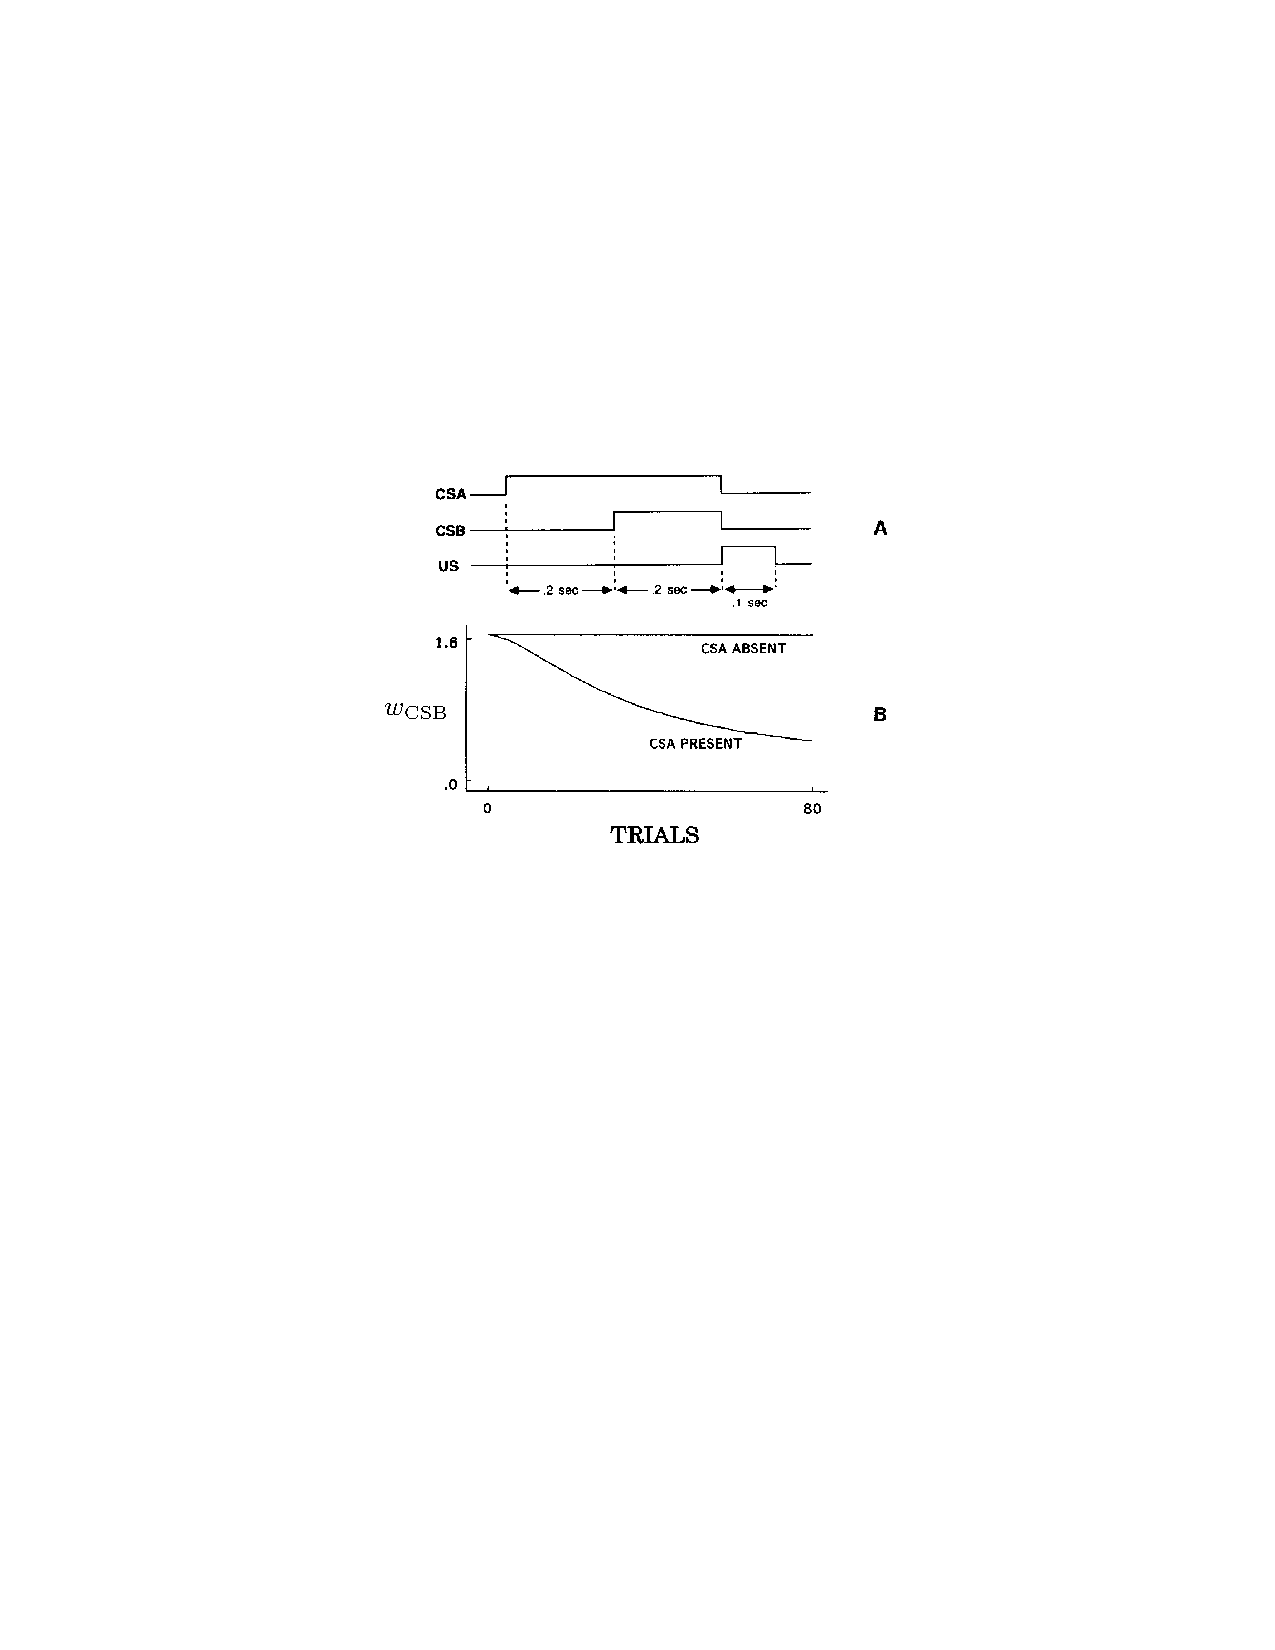
\includegraphics[width=0.5\linewidth]{chap11/fig_11_4}
	\caption{\textit{时间差分}模型中的时间优先覆盖阻塞。
		上图:刺激之间的时间关系。
		下图:当CSB有或没有CSA时,CSB的结合强度试验的行为。
		该模拟与图14.3所示的唯一不同之处在于,这里CSB开始完全调节| CSB的结合强度最初设置为1.653,当CSB单独用于80次试验时达到的最终水平,如图14.3中的“CSA缺席”情况。
		改编自Sutton和Barto(1990)。 \label{fig:11_4}}
\end{figure}


对于\textit{时间差分}模型,较早的预测刺激优先于较晚的预测刺激,因为与本书中描述的所有预测方法一样,\textit{时间差分}模型基于backingup或bootstrapping思想:关联强度的更新将特定状态下的强度转移到较晚状态下的强度。
自举的另一个结果是\textit{时间差分}模型提供了高阶条件反射的解释,这是经典条件反射的一个特征,超出了\textit{雷斯科拉-瓦格纳模型}和类似模型的范围。
如上所述,高阶条件反射是一种现象,其中先前条件反射的\textit{条件刺激}可以充当\textit{非条件刺激}来调节另一个最初中性的刺激。
图~\ref{fig:11_5}~显示了\textit{时间差分}模型(同样具有存在表示)在高阶调节实验中的行为,在这种情况下,它是二阶调节。
在第一阶段(图中未显示),CSB被训练来预测\textit{非条件刺激},以便其关联强度增加,此处为1.6。
在第二阶段,在没有\textit{非条件刺激}的情况下,CSA与CSB配对,顺序排列如图顶部所示。
即使CSA从未与\textit{非条件刺激}配对,它也会获得结合强度。
随着持续的训练,CSA的结合强度达到峰值,然后下降,因为二次增强剂CSB的结合强度降低,从而失去了提供二次增强的能力。
CSB的结合强度降低,因为\textit{非条件刺激}在这些高阶条件试验中没有发生。
这些是CSB的灭绝试验,因为它与\textit{非条件刺激}的预测关系被破坏,因此其作为增强剂的能力下降。
在动物实验中也可以看到同样的模式。
在高阶调节试验中,条件强化的这种消失使得很难证明高阶调节,除非通过偶尔插入一阶试验定期刷新原始预测关系。


\begin{figure}[!htb]
	\centering
	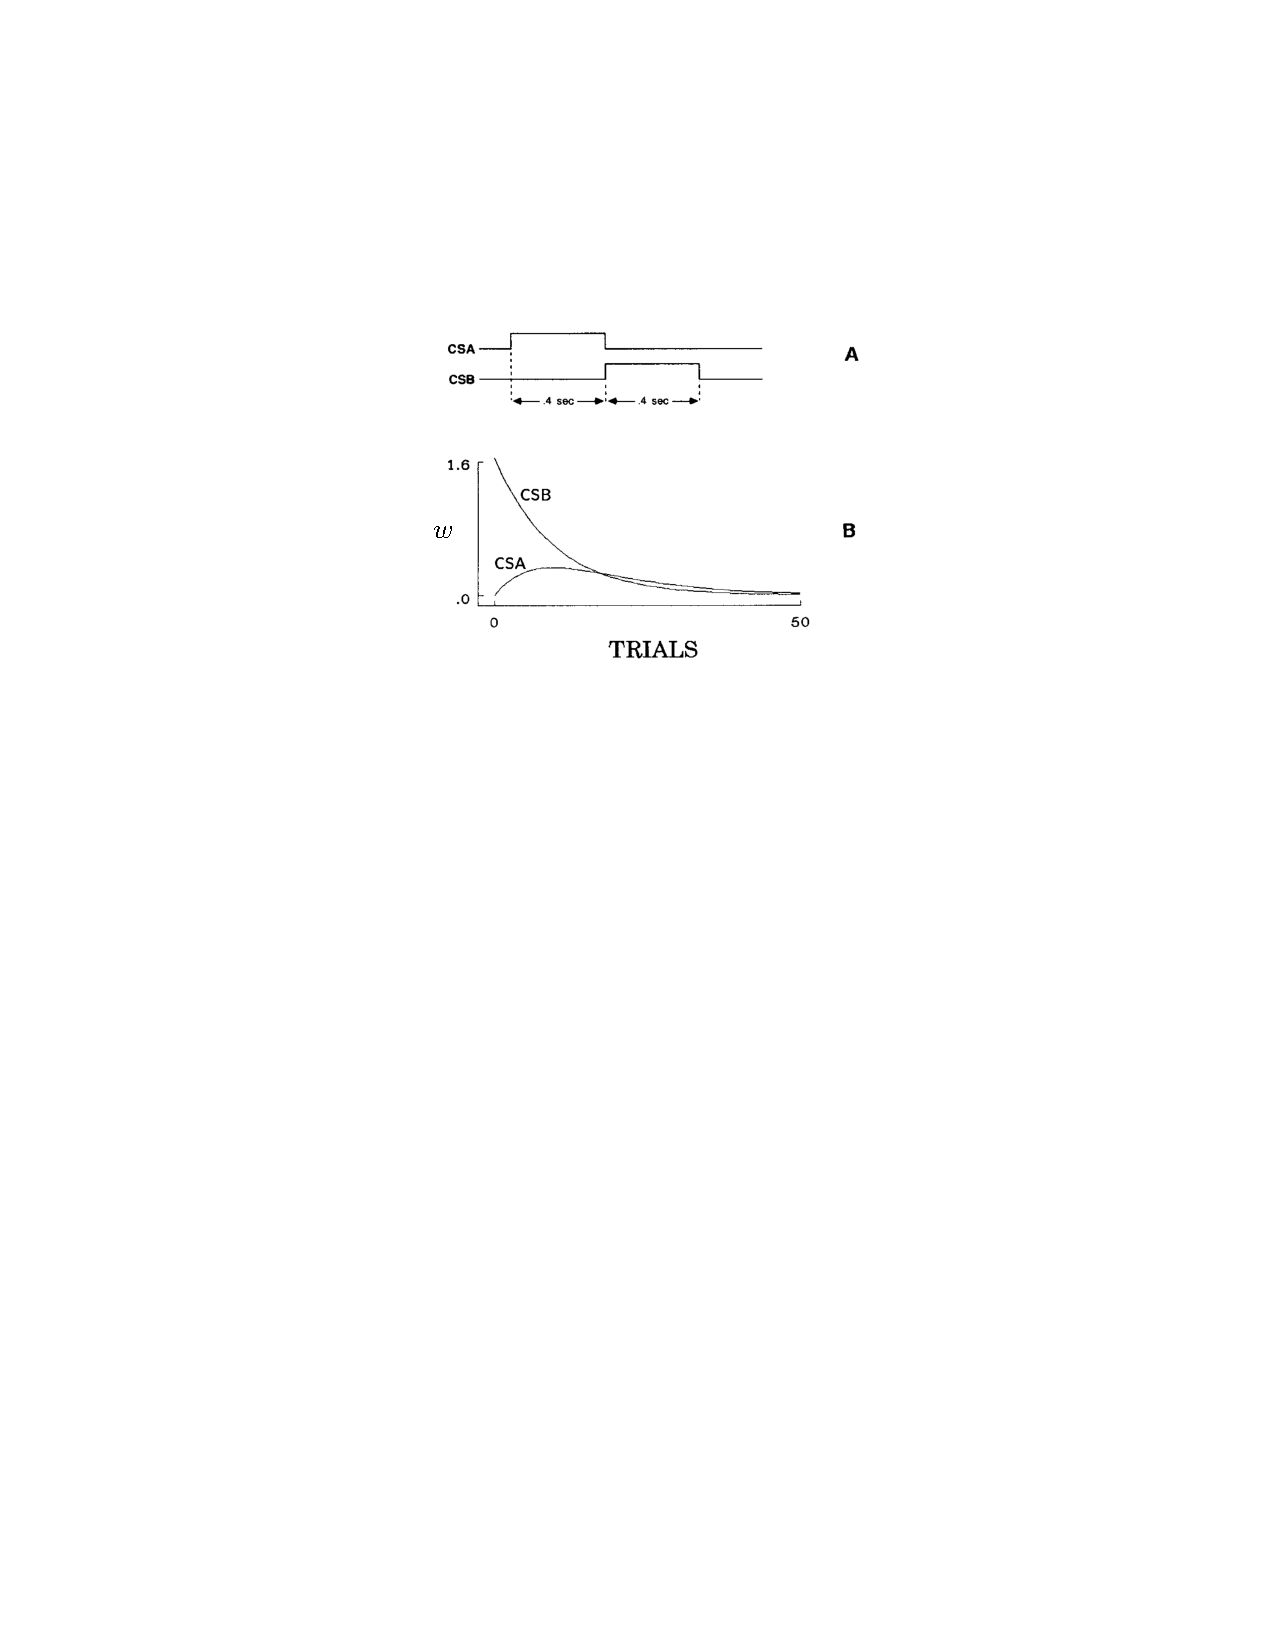
\includegraphics[width=0.5\linewidth]{chap11/fig_11_5}
	\caption{\textit{时间差分}模型的二阶调节。
		上图:刺激之间的时间关系。
		下图:与CSA和CSB相关的联合强度在试验中的行为。
		第二个刺激CSB在模拟开始时的初始关联强度为1.653。
		改编自Sutton和Barto(1990)。 \label{fig:11_5}}
\end{figure}


\textit{时间差分}模型产生了二阶和高阶条件的模拟,因为 v(St+1;wt)v(St;wt)出现在\textit{时间差分}错误t(14.5)中。这意味着作为先前学习的结果, v(St+1;wt)可以与 v(St;wt)分开,使得t非零(时间差异)。这种差异与(14.5)中的Rt+1具有相同的状态,这意味着就学习而言,时间差异和\textit{非条件刺激}的发生之间没有差异。
事实上,\textit{时间差分}算法的这一特征是其发展的主要原因之一,我们现在通过第6章所述的与动态规划的联系来理解它。自举值与二阶和高阶条件密切相关。


在上述\textit{时间差分}模型行为的示例中,我们仅检查了\textit{条件刺激}组件的关联强度的变化;
我们没有研究该模型对动物\textit{条件反射}特性的预测:它们的时间,形状以及它们如何发展过度条件反射试验。
这些特性取决于物种,观察到的反应系统以及调理试验的参数,但是在许多使用不同动物和不同反应系统的实验中,\textit{条件反射}的大小或\textit{条件反射}的概率随着\textit{非条件刺激}的预期时间的接近而增加。
例如,在我们上面提到的兔子的切口膜反应的经典调理中,过度调理试验从\textit{条件刺激}开始到切口膜开始穿过眼睛的延迟在试验中减少,并且这种预期闭合的幅度在\textit{条件刺激}和\textit{非条件刺激}之间的间隔内逐渐增加,直到膜在\textit{非条件刺激}的预期时间达到最大闭合。
这种\textit{条件反射}的时间和形状对于其适应性意义至关重要|过早覆盖眼睛会降低视力(即使切口膜是半透明的),而太晚覆盖它几乎没有保护价值。
对于经典调节模型来说,捕获这样的\textit{条件反射}特征具有挑战性。


\textit{时间差分}模型不包括任何将\textit{非条件刺激}预测的时间过程 v(St;wt)转换为可以与动物\textit{条件反射}特性进行比较的过程的机制。
最简单的选择是让模拟\textit{条件反射}的时间过程等于\textit{非条件刺激}预测的时间过程。
在这种情况下,模拟\textit{条件反射}的特征及其在试验中的变化方式仅取决于所选的刺激表示以及模型参数的值,和。


图~\ref{fig:11_6}~显示了学习过程中不同时间点\textit{非条件刺激}预测的时间过程,图~\ref{fig:11_1}~中显示了三种表示。
对于这些模拟,\textit{非条件刺激}在\textit{条件刺激}发作后发生了25个时间步长,并且=:05,=:95和=:97。使用CSC表示(图~\ref{fig:11_6}~左),\textit{时间差分}模型形成的\textit{非条件刺激}预测曲线在\textit{条件刺激}和\textit{非条件刺激}之间的整个间隔内呈指数增长,直到它在\textit{非条件刺激}发生时达到最大值(在时间步骤25)。
这种指数增长是\textit{时间差分}模型学习规则折扣的结果。对于存在表示(图~\ref{fig:11_6}~中),当刺激存在时,\textit{非条件刺激}的预测几乎是恒定的,因为每个刺激只有一个权重或关联强度需要学习。
因此,具有存在表示的\textit{时间差分}模型不能重建\textit{条件反射}定时的许多特征。
使用\textit{微刺激}表示(右图~\ref{fig:11_6}),\textit{时间差分}模型的\textit{非条件刺激}预测的发展更加复杂。
经过200次试验后,预测的曲线是用CSC表示产生的\textit{非条件刺激}预测曲线的合理近似值。


\begin{figure}[!htb]
	\centering
	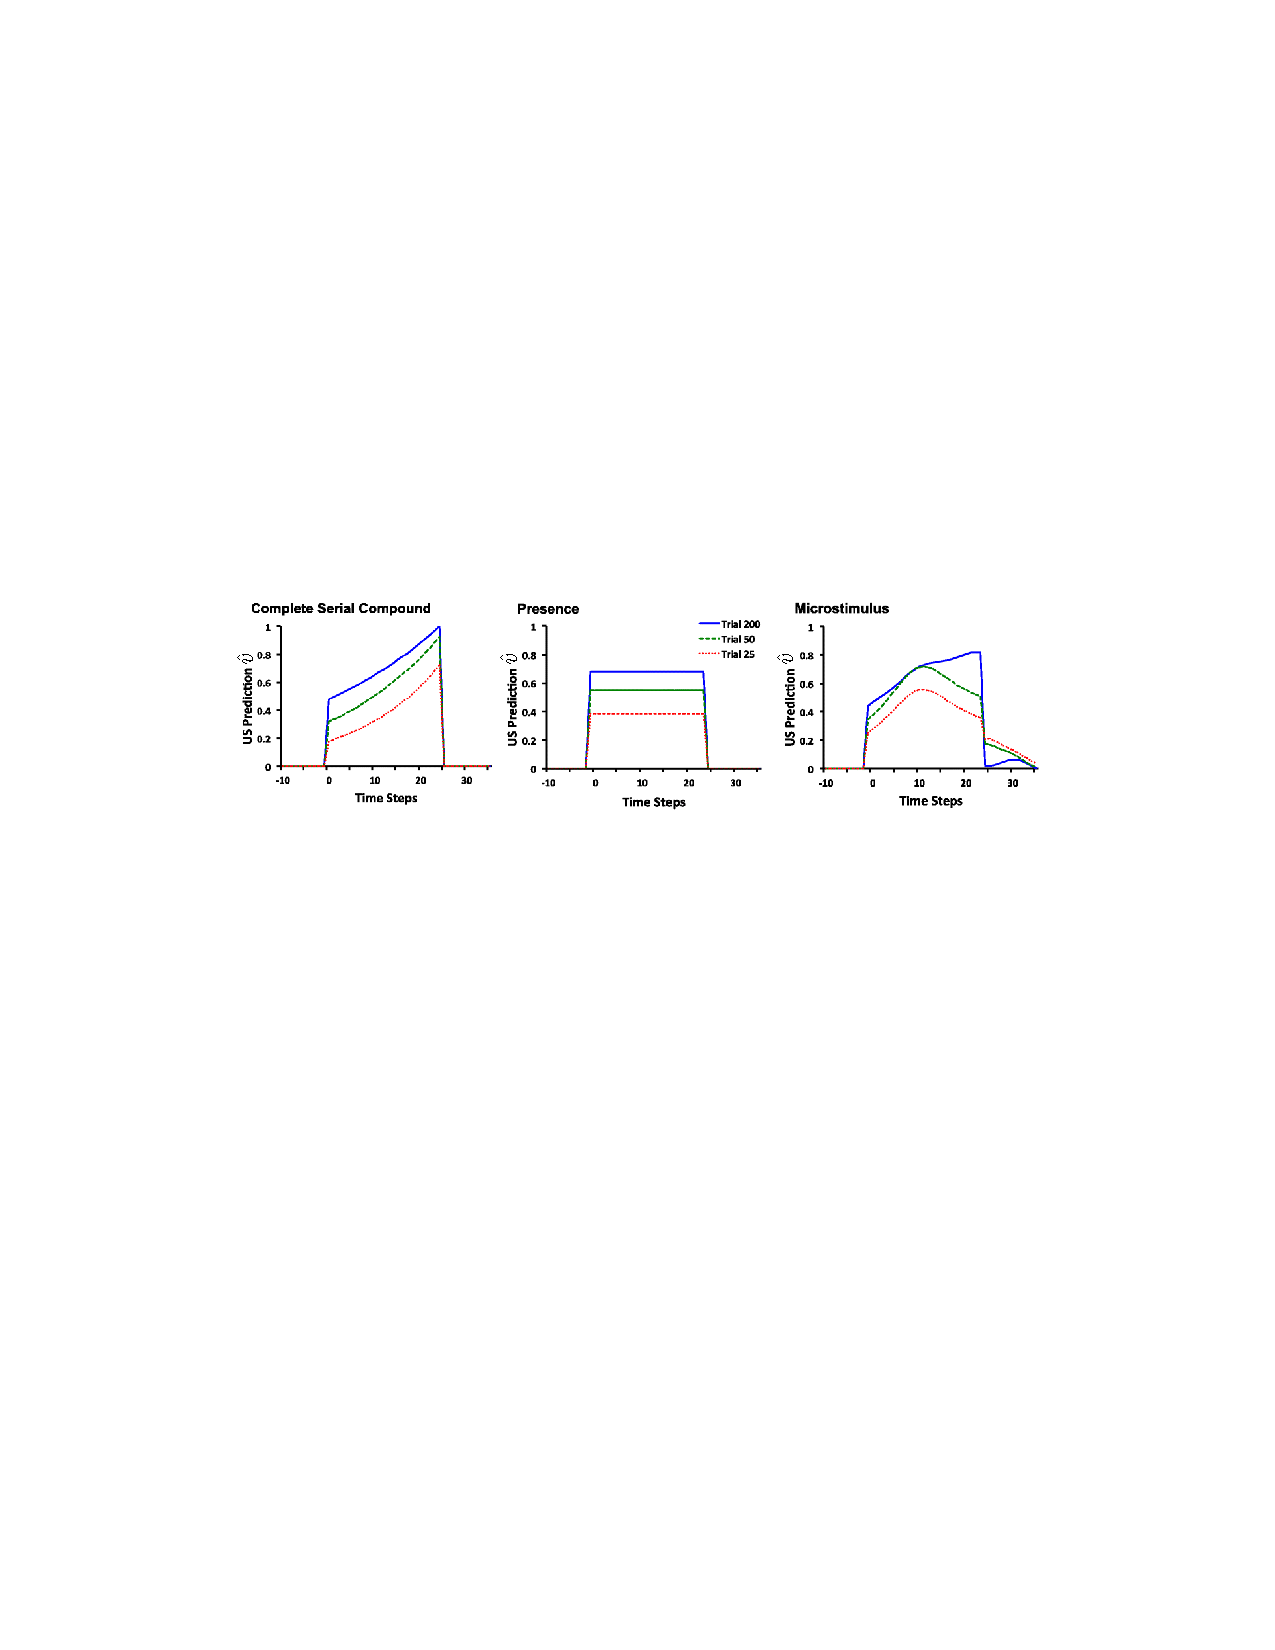
\includegraphics[width=0.8\linewidth]{chap11/fig_11_6}
	\caption{具有三种不同刺激表示的\textit{时间差分}模型在获取过程中\textit{非条件刺激}预测的时间过程。
		左:对于完整序列化合物(CSC),\textit{非条件刺激}预测在整个间隔内呈指数增长,在\textit{非条件刺激}时间达到峰值。
		在渐近线(试验200),\textit{非条件刺激}预测在\textit{非条件刺激}强度达到峰值(这些模拟中为1)。
		中间:通过存在表示,\textit{非条件刺激}的预测收敛到几乎恒定的水平。
		这个恒定水平由\textit{非条件刺激}强度和\textit{条件刺激} \textit{非条件刺激}间隔的长度决定。
		右:使用微刺激表示,在渐近线处,\textit{时间差分}模型通过不同微刺激的线性组合近似于CSC描绘的指数增长的时间过程。\label{fig:11_6}}
\end{figure}
			
			
图~\ref{fig:11_6}~所示的\textit{非条件刺激}预测曲线并不是为了精确匹配\textit{条件反射}在任何特定动物实验中调节过程中产生的曲线,但它们说明了刺激表示对\textit{时间差分}模型得出的预测的强烈影响。
此外,尽管我们只能在这里提到,但刺激表现如何与折扣和资格痕迹相互作用,对于确定\textit{时间差分}模型产生的\textit{非条件刺激}预测曲线的性质很重要。
我们在这里可以讨论的另一个方面是将我们的预测转化为\textit{条件反射}-proles的不同响应生成机制的影响;
图~\ref{fig:11_6}~所示的pro-les是“原始的”\textit{非条件刺激}预测pro-les。
即使没有任何关于动物大脑如何从\textit{非条件刺激}预测中产生明显反应的特殊假设,但是,图~\ref{fig:11_6}~中CSC和\textit{微刺激}表示的pro-les随着\textit{非条件刺激}时间的接近而增加,并在\textit{非条件刺激}时间达到最大值,正如许多动物调节实验所见。


\textit{时间差分}模型与特定的刺激表征和反应产生机制相结合,能够解释在动物经典条件反射实验中观察到的令人惊讶的广泛现象,但它远不是一个完美的模型。
为了生成经典调节的其他细节,需要扩展模型,也许可以通过添加基于模型的元素和机制来自适应地改变其某些参数。
建模经典条件反射的其他方法与\textit{雷斯科拉-瓦格纳模型}风格的误差校正过程明显不同。
例如,贝叶斯模型在概率框架内工作,经验可以修改概率估计。
所有这些模型都有助于我们理解经典条件反射。


也许\textit{时间差分}模型最显着的特点是它基于一种理论,即我们在本书中描述的理论,该理论表明动物的神经系统在经历条件反射时试图做什么:
它试图形成准确的长期预测,与刺激表现方式和神经系统如何工作所施加的限制相一致。
换句话说,它提出了经典条件反射的规范性解释,其中长期而不是即时的预测是一个关键特征。


经典条件反射\textit{时间差分}模型的发展就是一个例子,其中明确的目标是模拟动物学习行为的一些细节。
因此,\textit{时间差分}学习除了作为一种算法的地位外,也是这种生物学习方面模型的基础。
正如我们在第15章中所讨论的,\textit{时间差分}学习也被证明是产生多巴胺的神经元活动的基础模型,多巴胺是哺乳动物大脑中的一种化学物质,与奖励处理密切相关。
在这些例子中,强化学习理论与动物行为和神经数据进行了详细的联系。


我们现在转向考虑强化学习和动物行为在仪器调节实验中的对应关系,这是动物学习心理学家研究的另一种主要类型的实验室实验。


\section{操作性条件反射} \label{sec:instrumental_conditioning}

在仪器调节实验中,学习取决于行为的后果:强化刺激的传递取决于动物的行为。
相比之下,在经典的条件反射实验中,强化刺激“\textit{非条件刺激}”是独立于动物的行为而传递的。
工具性条件反射通常被认为与操作性条件反射相同,术语是为行为偶然强化实验引入的\cite{skinner2019behavior},尽管使用这两个术语的人的实验和理论在许多方面有所不同,其中一些我们将在下面讨论。
我们将专门使用术语仪器调节来进行实验,其中强化取决于行为。
工具性条件反射的根源可以追溯到\textit{非条件刺激}心理学家\textit{爱德华$\cdot$李$\cdot$桑代克}在本书第一版出版前100年进行的实验。


\textit{桑代克}观察到猫被放在拼图盒中时的行为,“它们可以通过适当的动作从拼图盒中逃生”(图~\ref{fig:11_7}~)。
例如,猫可以通过执行三个独立的动作来打开一个盒子的门:
按下盒子后面的平台,用爪子拉绳子,然后上下推一根横杆。
当第一次放在拼图盒中,外面可以看到食物时,除了少数几只\textit{桑代克}的猫外,所有猫都表现出明显的不适迹象“和异常剧烈的活动,本能地努力逃离困境”\cite{thorndike1898animal}。


\begin{figure}[!htb]
	\centering
	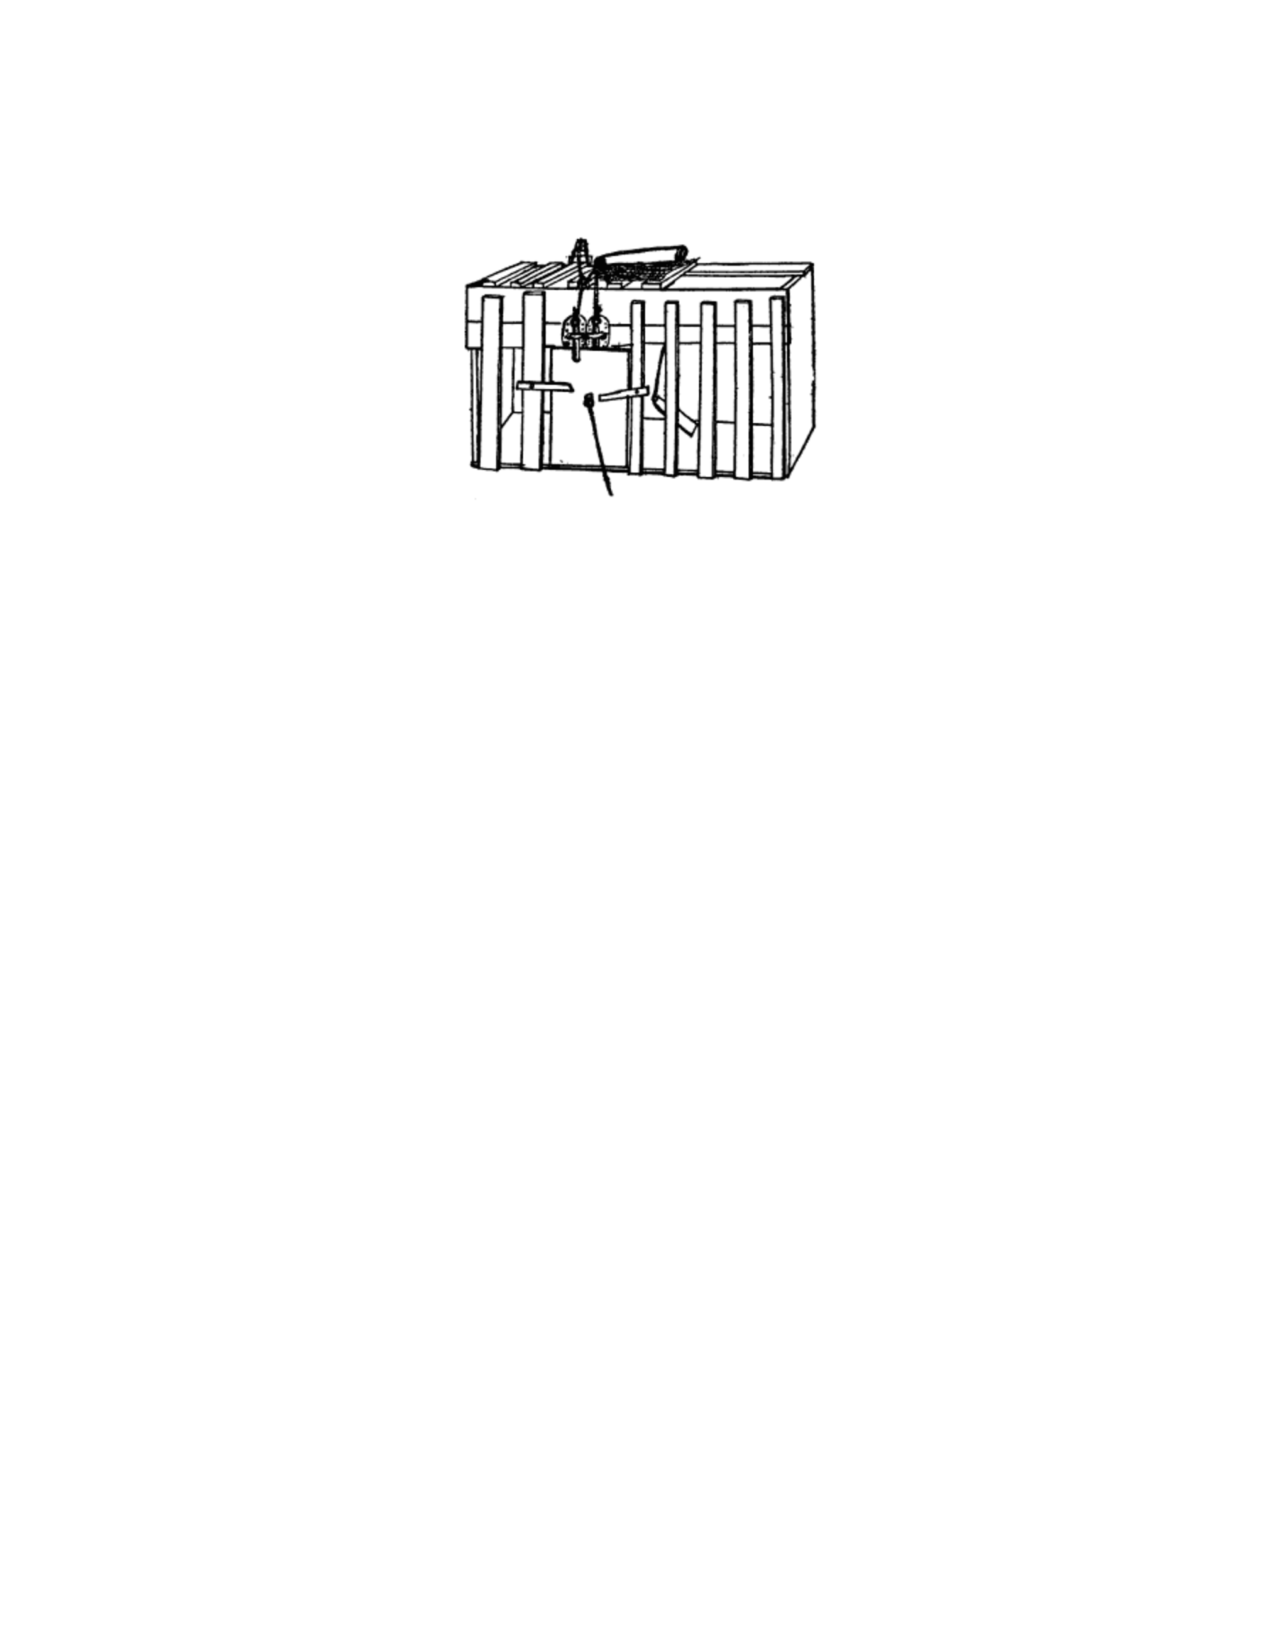
\includegraphics[width=0.5\linewidth]{chap11/fig_11_7}
	\caption{\textit{桑代克}的一个拼图盒\cite{thorndike1898animal}。  \label{fig:11_7}}
\end{figure}

在对不同的猫和具有不同逃生机制的盒子进行的实验中,\textit{桑代克}记录了每只猫在每个盒子中多次逃生所花费的时间。
他观察到,时间几乎总是随着连续的经历而减少,例如从300秒减少到6或7秒。
他在一个拼图框中描述了猫的行为,如下所示:


在冲动的挣扎中,一只猫在盒子上抓来抓去,它很可能会抓住绳子、环或按钮来开门。
渐渐地,所有其他不成功的冲动都会被消除,导致成功行为的特定冲动会被由此产生的快乐所抑制,直到经过多次尝试后,猫被放入盒子后,会立即以一种明确的方式抓住按钮或回路\cite{thorndike1898animal}。


这些和其他实验(一些是针对狗,小鸡,猴子,甚至sh)导致\textit{桑代克}制定了许多学习的“定律”,其中最重要的是电子定律,我们在第一章中引用了它的一个版本。
这条定律描述了通常所说的通过试错学习。
如第1章所述,ect法的许多方面都产生了争议,多年来其细节已经被修改。
尽管如此,法律以某种形式表达了一种持久的学习原则。


强化学习算法的基本特征对应于ect定律描述的动物学习特征。
首先,强化学习算法是选择性的,这意味着它们会尝试替代方案,并通过比较其结果来进行选择。
其次,强化学习算法是关联的,这意味着通过选择找到的替代方案与特定情况或状态相关联,以形成代理的策略。
就像效应定律描述的学习一样,强化学习不仅是发现产生大量奖励的行为的过程,而且是将这些行为与情境或状态联系起来的过程。
\textit{桑代克}使用了短语“通过选择和连接学习”。
进化中的自然选择是选择过程的一个主要例子,但它不是关联的(至少正如人们普遍理解的那样);
监督学习是关联的,但它不是选择的,因为它依赖于直接告诉代理人如何改变其行为的指令。


从计算的角度来看,ect定律描述了一种将搜索和记忆结合起来的基本方法:
在每种情况下,以尝试和选择许多动作的形式进行搜索,并以将情景与迄今为止发现的动作联系起来的关联形式进行记忆,以便在这些情况下发挥最佳作用。
搜索和记忆是所有强化学习算法的重要组成部分,无论记忆是以代理的策略、价值函数还是环境模型的形式出现。


强化学习算法需要搜索意味着它必须以某种方式进行探索。
动物也很清楚地探索,早期的动物学习研究人员不同意动物在\textit{桑代克}的拼图盒等情况下选择行为的指导程度。
行动是绝对随机、盲目摸索的结果吗?(Woodworth,1938,第777页),还是有某种程度的指导,无论是来自先前的学习、推理还是其他手段?
尽管包括\textit{桑代克}在内的一些思想家似乎采取了前一种立场,但其他人则倾向于更深思熟虑的探索。
强化学习算法允许在选择行动时有很大的自由度。
我们在本书中介绍的算法中使用的探索形式,如贪婪和上限行为选择,只是最简单的。
更复杂的方法是可能的,唯一的规定是必须有某种形式的探索才能使算法有效工作。


我们处理强化学习的特点是允许随时可用的一组动作取决于环境的当前状态,这与\textit{桑代克}在他的猫的拼图盒行为中观察到的情况相呼应。
猫从它们在当前情况下本能地执行的动作中选择动作,\textit{桑代克}称之为“本能冲动”。
“首先放在一个拼图盒中,猫会本能地抓挠、抓抓和咬,充满活力:
猫对自己在一个有限的空间中行走的本能反应。
成功的动作是从这些动作中选择的,而不是从每一个可能的动作或活动中选择。
这就像我们形式主义的特征,从一个状态s中选择的动作属于一组可接受的动作a(s)。指定这些动作是强化学习的一个重要方面,因为它可以从根本上简化学习。
它们就像动物的本能冲动。
另一方面,\textit{桑代克}的猫可能是根据一种特定于动作的本能上下文顺序进行探索的,而不仅仅是从一组动作中进行选择。
本能冲动。这是另一种使强化学习更容易的方法。


克拉克·赫尔(Clark Hull,例如赫尔,1943年)和B.F.斯金纳\cite{skinner2019behavior}是受ect定律影响最杰出的动物学习研究人员之一。
他们研究的核心是根据后果选择行为的想法。
强化学习与赫尔理论有着共同的特征,其中包括类似资格的机制和二次强化,以解释在动作与随后的强化刺激之间存在显着的时间间隔时学习的能力(见第14.4节)。
随机性也在赫尔的理论中发挥了作用,他称之为“行为振荡”来引入探索行为。


斯金纳并没有完全赞同ect定律的记忆方面。他反对联想联系的想法,而是强调从自发产生的行为中进行选择。
他引入“操作性”一词来强调动作对动物环境的关键作用。
与\textit{桑代克}等人的实验不同,斯金纳的操作性条件反射实验允许动物受试者长时间不间断地行为。
他发明了操作性条件反射室,现在称为“斯金纳盒,“最基本的版本包含一个杠杆或钥匙,动物可以按下它来获得奖励,如食物或水,这些奖励将根据一个明确的规则传递,称为强化时间表。
通过记录杠杆按压的累积次数作为时间的函数,斯金纳和他的追随者可以研究不同强化时间表对动物杠杆按压速度的影响。
使用我们在本书中介绍的强化学习原则对类似实验的建模结果并不完善,但我们在本章末尾的书目和历史评论部分提到了一些例外。


斯金纳的另一个贡献来自于他认识到通过加强对所需行为的连续近似来训练动物的有效性,他称之为塑造过程。
虽然这项技术已经被包括斯金纳本人在内的其他人使用过,但当他和同事试图用鸟嘴刷木球训练鸽子打保龄球时,这项技术的重要性给他留下了深刻的印象。
在等待了很长时间而没有看到任何可以加固的刷子之后,他们


…决定加强任何与刷球最相似的反应,也许一开始只是看球的行为,然后选择更接近最终形式的反应。结果令我们惊讶。几分钟后,球在盒子的墙上旋转,就像鸽子是壁球冠军一样。(斯金纳,1958年,第94页)


鸽子不仅学会了一种对鸽子来说不寻常的行为,而且还通过一个互动过程快速学会了,在这个过程中,它的行为和强化突发事件会随着对方的反应而改变。
斯金纳将改变强化偶然性的过程与雕塑家将粘土塑造成所需形式的工作进行了比较。
塑造也是计算强化学习系统的强大技术。
当一个代理很难接收到任何非零奖励信号时,无论是由于奖励情况的稀疏性还是由于初始行为的不可接近性,从一个更容易的问题开始,随着代理的学习逐渐增加其难度可能是一种有效的,有时是必不可少的策略。


心理学中一个与工具性条件作用特别相关的概念是动机,它指的是影响行为方向和力量或活力的过程。
例如,\textit{桑代克}的猫就有动力逃离拼图盒,因为它们想要坐在外面的食物。
实现这一目标对他们来说是有益的,并加强了允许他们逃跑的行动。
很难将具有多个维度的动机概念精确地与强化学习的计算观点联系起来,但它与某些维度有明确的联系。


从某种意义上说,强化学习代理的奖励信号是其动机的基础:
从长远来看,代理的动机是最大化其获得的总奖励。
因此,动机的一个关键方面是,是什么使代理人的经验获得回报。
在强化学习中,奖励信号取决于强化学习代理的环境状态和代理的行为。
此外,正如第1章所指出的,代理环境的状态不仅包括关于机器外部的信息,如容纳代理的生物体或机器人,还包括机器内部的信息。
一些内部状态成分对应于心理学家所说的动物的动机状态,这会影响对动物的奖励。
例如,一只动物饥饿时吃东西比刚吃完一顿令人满意的饭时会得到更多的回报。
状态依赖的概念足够广泛,可以对奖励信号的产生产生多种类型的调制影响。


价值函数为心理学家的动机概念提供了进一步的联系。
如果选择行动的最基本动机是获得尽可能多的奖励,那么对于使用价值函数选择行动的强化学习代理来说,更接近的动机是提升其价值函数的梯度,即选择预期会导致最有价值的下一个状态的行动(或者本质上相同的事情,选择具有最大行动价值的行动)。
对于这些代理人来说,价值函数是决定其行为方向的主要驱动力。


动机的另一个维度是,动物的动机状态不仅影响学习,而且影响动物学习后行为的强度或活力。
例如,在学习在迷宫的目标框中寻找食物后,饥饿的老鼠比不饥饿的老鼠跑得更快。
动机的这一方面并没有与我们在这里介绍的强化学习框架如此清晰地联系起来,但在本章末尾的书目和历史评论部分,我们引用了几篇提出基于强化学习的行为活力理论的出版物。


我们现在转向学习的主题,当强化刺激发生在它们强化的事件之后。
强化学习算法使用的机制能够通过延迟强化进行学习|资格痕迹和\textit{时间差分}学习|与心理学家关于动物在这些条件下如何学习的假设密切相关。


\section{延迟强化}


\textit{效果律}要求在联系上有一个向后的效果,一些早期的法律批评者无法想象现在如何能够影响过去的事情。
这种担忧加剧了这样一个事实,即当行动与随之而来的奖励或惩罚之间存在相当大的延迟时,甚至可以进行学习。
同样,在经典条件反射中,当\textit{非条件刺激}发作遵循\textit{条件刺激} o设定的不可忽略的时间间隔时,可能会发生学习。
我们称之为延迟强化问题,这与Minsky\cite{minsky1961steps}所称的学习系统的信用分配问题有关:你如何在可能涉及产生成功的许多决策中分配成功的信用?
本书中介绍的强化学习算法包括两种解决此问题的基本机制。
第一种是使用资格痕迹,第二种是使用\textit{时间差分}方法学习价值函数,这些价值函数可以提供近乎即时的行为评估(在仪器调节实验等任务中)或提供即时的预测目标(在经典调节实验等任务中)。
这两种方法都对应于动物学习理论中提出的类似机制。


巴甫洛夫(1927)指出,每个刺激都必须在刺激结束后的一段时间内在神经系统中留下痕迹,他提出,当\textit{条件刺激}o集和\textit{非条件刺激}发病之间存在时间差距时,刺激痕迹使学习成为可能。
直到今天,在这些条件下的调节被称为痕量调节(第285页)。
假设当\textit{非条件刺激}到达时,\textit{条件刺激}的痕迹仍然存在,学习是通过痕迹和\textit{非条件刺激}的同时存在而发生的。
我们在第15章讨论了一些关于神经系统痕迹机制的建议。


刺激痕迹也被提议作为一种手段,用于弥合仪器调节中动作与随之而来的奖惩之间的时间间隔。
例如,在赫尔的内在学习理论中,“摩尔刺激痕迹”解释了他所谓的动物的目标梯度,描述了仪器条件反应的最大强度如何随着强化延迟的增加而降低(赫尔,19321943)。
赫尔假设动物的动作会留下内部刺激,自采取动作以来,其痕迹会随着时间呈指数衰减。
查看当时可用的动物学习数据,他假设痕迹在30到40秒后有效地达到零。




本书中描述的算法中使用的合格性迹线类似于赫尔迹线:它们是过去状态访问或过去状态{动作对的衰减迹线。
合格性迹线是由Klopf\cite{klopf1972brain}在他的神经元理论中引入的,在他的神经元理论中,它们是突触中过去活动的时间扩展迹线,即神经元之间的连接。
Klopf的迹线比我们算法使用的指数衰减迹线更复杂,当我们在第15.9节中学习他的理论时,我们会对此进行更多讨论。


为了解释比刺激痕迹跨越更长时间的目标梯度,赫尔(1943)提出,更长的梯度是由从目标向后传递的条件强化产生的,这一过程与他的摩尔刺激痕迹一起起作用。
动物实验表明,如果条件有利于在延迟期间发展条件性强化,那么学习不会像在阻碍二次强化的条件下那样随着延迟的增加而减少。
如果在延迟间隔期间有规律发生的刺激,则有条件的强化是有利的。
然后,似乎奖励实际上并没有延迟,因为有更直接的条件强化。
因此,赫尔设想,基于刺激痕迹介导的初级强化的延迟,存在一个初级梯度,并且通过条件性强化逐渐修改和延长。


本书中提出的算法使用资格跟踪和价值函数来实现延迟强化学习,这与赫尔关于动物在这些条件下如何学习的假设相对应。
\textit{行动者}第13.5节、第15.7节和第15.8节中讨论的\textit{评论家}体系结构最清楚地说明了这种对应关系。
\textit{评论家}使用\textit{时间差分}算法学习与系统当前行为相关的值函数,即预测当前策略的返回。
参与者根据\textit{评论家}的预测更新当前策略,或者更准确地说,根据\textit{评论家}预测的变化更新当前策略。
\textit{评论家}产生的\textit{时间差分}误差充当了参与者的条件强化信号,即使主要奖励信号本身被大大延迟,也能立即评估性能。
估计动作值函数的算法,例如Q学习和Sarsa,类似地使用\textit{时间差分}学习原理,通过条件强化来实现延迟强化学习强化。
我们在第15章中讨论的\textit{时间差分}学习与产生多巴胺的神经元的活动之间的紧密平行,为强化学习算法与赫尔的这一方面之间的联系提供了额外的支持收益理论。


\section{认知地图} \label{sec:cognitive_maps}

基于模型的强化学习算法使用的环境模型与心理学家所称的认知图具有共同的元素。
回想一下我们在第8章中对规划和学习的讨论,环境模型指的是代理人可以用来预测其环境在状态转换和奖励方面如何响应其行为的任何东西,而规划指的是从这样的模型计算策略的任何过程。
环境模型由两部分组成:状态转换部分编码关于行为对状态变化的影响的知识,奖励模型部分编码关于每个状态或每个状态{动作对{预期的奖励信号的知识。
基于模型的算法通过使用模型来选择动作,以根据未来状态和预期从这些状态产生的奖励信号来预测可能的行为过程的后果。
最简单的计划是比较“想象”决策序列集合的预测后果。


关于动物是否使用环境模型的问题,如果是这样的话,模型是什么样的,它们是如何学习的,在动物学习研究的历史上起着至关重要的作用。
一些研究人员通过展示潜在学习,挑战了当时流行的\textit{刺激反应}学习和行为观,这与最简单的无模型学习策略相对应。
在最早的潜在学习实验中,两组大鼠在迷宫中跑步。
对于实验组来说,在实验的第一阶段没有奖励,但在第二阶段开始时食物突然被引入迷宫的目标框中。
对于对照组来说,食物在两个阶段都在目标框中。
问题是,在没有食物奖励的情况下,实验组的大鼠在第一阶段是否会学习到任何东西。
尽管实验大鼠在第一阶段似乎学习不多,但没有回报Ed,第二阶段,他们一发现第二阶段引入的食物,就迅速赶上了对照组的老鼠。
得出的结论是,在非奖励期,[实验组]的老鼠他们正在开发一种潜在的迷宫学习方法,一旦引入奖励,他们就能够利用这种方法”\cite{blodgett1929effect}。



潜在学习与心理学家爱德华·托尔曼(Edward Tolman)以及其他类似的人联系最为密切,托尔曼(Edward Tolman)将这一结果解释为表明动物可以在没有奖励或惩罚的情况下学习环境的认知地图,并且当他们有动机达到目标时,他们可以稍后使用该地图\cite{tolman1948cognitive}。
认知地图还可以让老鼠规划通往目标的路线,这与老鼠在最初探索中使用的路线不同。
对这些结果的解释导致了心理学中行为主义/认知二分法核心的持久争议。
现代意义上,认知地图不仅限于空间布局模型,更普遍的是环境模型或模型动物的任务空间”(例如,Wilson,Takahashi,Schoenbaum和Niv,2014)。
潜在学习实验的认知图解释类似于动物使用基于模型的算法的说法,并且即使没有明确的奖励或惩罚也可以学习环境模型。
然后,当动物受到奖励或惩罚的激励时,模型被用于计划。


托尔曼(Tolman)对动物如何学习认知图的描述是,它们通过在探索环境时经历刺激的连续性来学习刺激-刺激或s{s关联。在心理学中,这被称为期望理论:给定s{s关联,刺激的发生会产生对下一个刺激的期望。
这很像控制工程师所说的系统识别,即从标记的训练示例中学习具有未知动力学的系统模型。
在最简单的离散时间版本中,训练示例是s{S0对,其中s是状态,S0是后续状态。
当观察到s时,模型会创建期望接下来将观察S0。对计划更有用的模型也涉及动作,因此示例类似于SA{S0,其中当动作a在状态s下执行时,S0是预期的。
了解环境如何产生回报也很有用。在这种情况下,例子是S{R或SA{R的形式,其中R是与S或SA对相关联的奖励信号。
这些都是监督学习的形式,通过这些形式,代理可以获得类似认知的地图,无论它在探索其环境时是否接收到任何非零奖励信号。


\section{习惯性和目标导向的行为} \label{sec:habitual_behavior}

无模型和基于模型的强化学习算法之间的区别对应于心理学家对学习行为模式的习惯性和目标导向控制之间的区别。
习惯是由适当的刺激触发的行为模式,然后或多或少地自动执行。
根据心理学家如何使用这个短语,目标导向行为是有目的的,因为它受目标价值以及行为与其后果之间关系的知识的控制。
习惯有时被认为是由先前的刺激控制的,而目标导向的行为被认为是由其后果控制的(Dickinson,19801985)。
目标导向控制的优点是,当环境改变对动物行为的反应方式时,它可以迅速改变动物的行为。
虽然习惯行为对习惯环境的输入反应迅速,但它无法快速适应环境的变化。
目标导向行为控制的发展可能是动物智力进化的一个重大进步。


图~\ref{fig:11_8}~说明了无模型和基于模型的决策策略在假设任务中的差异,在该任务中,老鼠必须在具有独特目标框的迷宫中导航,每个目标框都提供了所示数量级的相关奖励(图~\ref{fig:11_8}~顶部)。
从S1开始,老鼠必须首先选择左(L)或右(R),然后必须在S2或S3再次选择L或R才能到达其中一个目标框。
目标框是老鼠情节任务每一集的终端状态。无模型策略(图~\ref{fig:11_8}~左下)依赖于状态{动作对的存储值。
这些动作值(Q值)是对大鼠从每个(非终点)状态采取的每个动作所能预期的最高回报的估计。
它们是通过多次从开始到结束运行迷宫的试验获得的。
当动作值对最佳回报的估计足够好时,大鼠只需在每个状态下选择动作值最大的动作即可做出最佳决策。
在这种情况下,当动作值估计足够准确时,大鼠从S1中选择L,从S2中选择R,以获得4的最大回报。
不同的无模型策略可能仅仅依赖于缓存的策略而不是操作值,从而实现从S1到L以及从S2到R的直接链接。
在这两种策略中,决策都不依赖于环境模型。
不需要参考状态转换模型,目标框的功能与它们提供的奖励之间也不需要连接。


图~\ref{fig:11_8}(右下)说明了基于模型的策略。它使用由状态转换模型和奖励模型组成的环境模型。
状态转换模型显示为决策树,奖励模型将目标框的独特特征与每个目标框中要找到的奖励相关联。
(与状态S1,S2和S3相关的奖励也是奖励模型的一部分,但这里它们是零,没有显示。)
基于模型的代理可以通过使用模型来模拟行动选择序列来决定在每个状态下转向哪种方式,以找到产生最高回报的路径。
在这种情况下,回报是从路径末尾的结果中获得的奖励。
在这里,使用足够精确的模型,大鼠将选择L,然后选择R以获得4的奖励。
比较模拟路径的预测收益是一种简单的规划形式,可以通过第8章讨论的多种方式完成。


当无模型代理的环境改变其对代理行为的反应方式时,代理必须在改变的环境中获得新的经验,在此期间可以更新其策略和/或价值函数。
例如,在图~\ref{fig:11_8}(左下)所示的无模型策略中,如果其中一个目标框以某种方式转变为提供不同的奖励,则老鼠将不得不穿过迷宫,可能需要多次才能在到达目标框时体验新的奖励,同时根据此经验更新其策略或其行动价值函数(或两者)。
关键的一点是,对于一个无模型的代理来说,要改变其策略为一个状态指定的动作,或者改变与一个状态相关的动作值,它必须移动到该状态,从该状态开始动作,可能多次,并经历其动作的后果。


\begin{figure}[!htb]
	\centering
	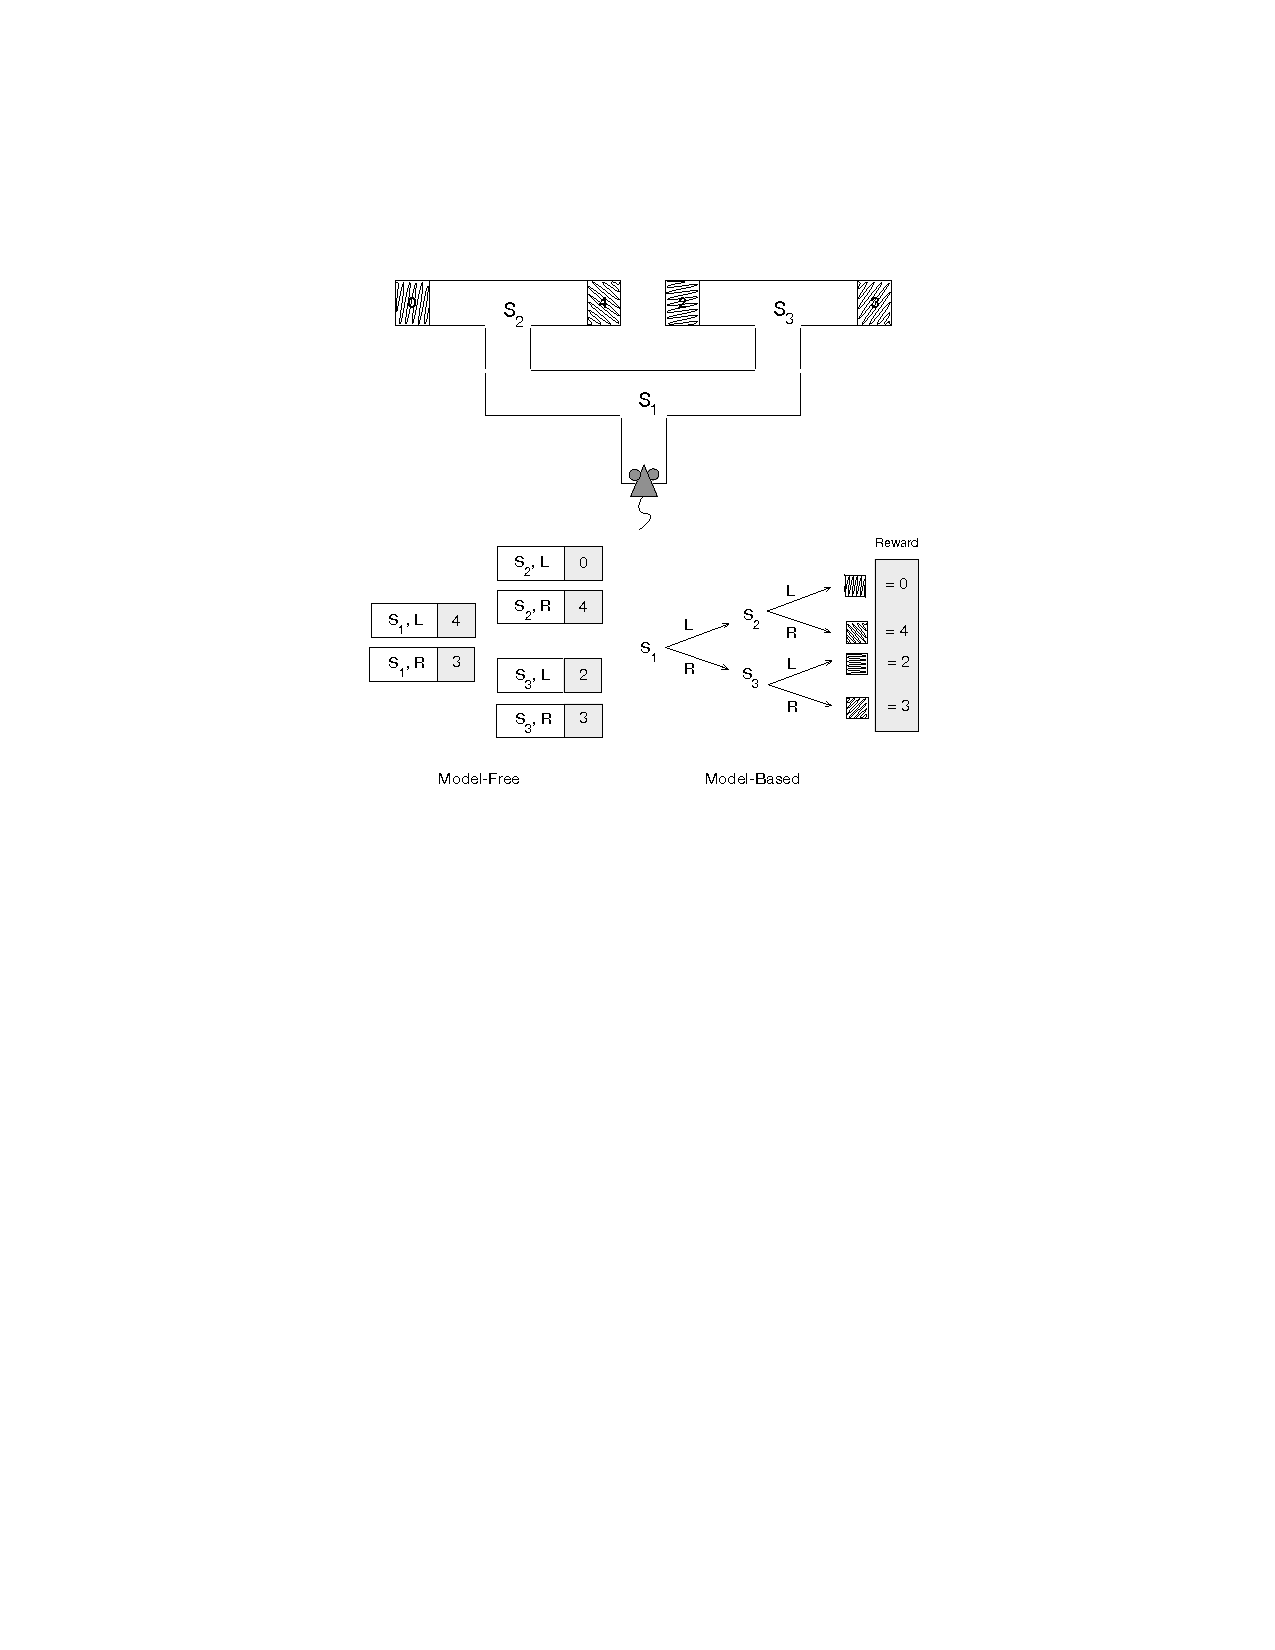
\includegraphics[width=0.65\linewidth]{chap11/fig_11_8}
	\caption{基于模型和无模型的策略来解决假设的顺序动作选择问题。
		上图:一只老鼠在迷宫中导航,迷宫中有独特的目标框,每个目标框都有一个显示值的奖励。
		左下:无模型策略依赖于在许多学习试验中获得的所有状态动作对的存储动作值。
		为了做出决策,大鼠只需在每个状态下选择该状态动作值最大的动作。
		右下:在基于模型的策略中,大鼠学习一个环境模型,该模型由状态动作-下一个状态转换的知识和一个奖励模型组成,该奖励模型由与每个独特目标框相关的奖励知识组成。
		大鼠可以通过使用该模型模拟动作选择的序列来决定在每个状态下转向哪种方式,从而找到产生最高回报的路径。
		改编自《认知科学趋势》,第10卷第8期,Y.Niv,D.Joel,和P.Dayan,《动机的规范观点》,第3762006页,经Elsevier许可。  \label{fig:11_8}}
\end{figure}


基于模型的代理可以适应其环境的变化,而不需要这种“个人经验”来了解变化所影响的状态和行为。
模型的更改(通过计划)会自动更改其策略。规划可以确定环境变化的后果,而这些变化在代理人自己的经历中从未联系在一起。
例如,再次参考图~\ref{fig:11_8}~中的迷宫任务,想象一只具有先前学习的过渡和奖励模型的老鼠直接放置在S2到nd右侧的目标框中,那里可用的奖励现在具有值1而不是4。
即使不涉及在迷宫中找到目标框所需的行动选择,老鼠的奖励模型也会改变。计划过程将为迷宫跑步带来新奖励的知识,而不需要额外的迷宫经验;
在这种情况下,在S1和S3处将策略更改为右转,以获得3的回报。


正是这种逻辑是动物结果贬值实验的基础。
这些实验的结果提供了一个洞察动物是否已经学会了一种习惯,或者它的行为是否处于目标导向的控制之下。
结果贬值实验类似于潜在的学习实验,因为奖励从一个阶段变为下一个阶段。
在学习的初始奖励阶段之后,结果的奖励值会发生变化,包括变为零甚至负值。


Adams和Dickinson(1981)进行了这种类型的早期重要实验。
他们通过仪器调节训练老鼠,直到老鼠在训练室中使劲按下蔗糖颗粒的杠杆。然后将大鼠放在同一个腔室中,杠杆缩回并允许非偶然食物,这意味着颗粒可以独立于它们的动作提供给它们。
在自由进入这些颗粒15分钟后,一组大鼠注射了引起恶心的有毒氯化锂。
重复三次,最后一次注射的大鼠都没有消耗任何非偶然性颗粒,这表明颗粒的奖励价值降低了,颗粒贬值了。
在一天后的下一个阶段,将大鼠再次放置在室内并进行一段时间的灭绝训练,这意味着响应杆回到原位但与颗粒分配器断开连接,以便按下它不会释放颗粒。
问题是,即使没有经历由于杠杆按压而贬值的奖励,那些颗粒奖励值降低的大鼠是否会比没有颗粒奖励值降低的大鼠杠杆按压更少。
事实证明,从灭绝试验开始,注射的大鼠的反应率明显低于未注射的大鼠。


亚当斯(Adams)和狄金森(Dickinson)得出结论,注射的大鼠通过将杠杆按压与颗粒和颗粒与恶心联系起来的认知图,将杠杆按压与随之而来的恶心联系起来。
因此,在灭绝试验中,老鼠知道“按下杠杆的后果是他们不想要的,因此他们从一开始就减少了杠杆的按压。
重要的是,他们减少了杠杆的按压,而没有经历过杠杆的按压直接伴随着生病:生病时没有杠杆。
他们似乎能够将行为选择的结果(按下杠杆之后会得到一个小球)的知识与结果的奖励值(小球是要避免的)结合起来,因此可以相应地改变他们的行为。
并不是每个心理学家都同意这种实验的认知解释,这不是解释这些结果的唯一可能的方法,而是模型基于规划的解释被广泛接受。


没有什么可以阻止代理同时使用无模型算法和基于模型的算法,并且有充分的理由同时使用这两种算法。
我们从自己的经验中知道,如果重复足够多,目标导向的行为往往会变成习惯性行为。实验表明,这种情况也发生在老鼠身上。
亚当斯(Adams,1982)进行了一项实验,以观察长期训练是否会将目标导向的行为转变为习惯性行为。
他通过比较经历不同训练量的大鼠结果贬值的影响来做到这一点。
如果与接受较少训练的大鼠相比,延长训练使大鼠对贬值的敏感性降低,这将证明延长训练使行为更加习惯。
亚当斯的实验紧跟着刚刚描述的亚当斯和狄金森(1981)的实验。简化一点,一组大鼠接受训练,直到他们做出100次奖励杠杆按压,另一组大鼠(过度训练组)接受训练,直到他们做出500次奖励杠杆按压。
训练后,两组大鼠的颗粒奖励值均降低(使用氯化锂注射)。
然后对两组大鼠进行一次灭绝训练。亚当斯的问题是,贬值是否会使过度训练的老鼠的杠杆按压率低于非过度训练的老鼠,这将证明延长训练会降低对结果贬值的敏感性。
结果表明,贬值大大降低了非过度训练大鼠的杠杆按压率。
相反,对于过度训练的老鼠来说,贬值对他们的杠杆按压几乎没有影响;事实上,如果有什么不同的话,它会使它更有活力。
(完整的实验包括对照组,表明不同程度的训练本身并没有显着影响学习后的杠杆按压率。)
这一结果表明,虽然非过度训练的大鼠以目标导向的方式行事,对他们的行为结果的知识敏感,但过度训练的大鼠已经养成了杠杆按压的习惯。



从计算的角度来看这个结果和其他类似的结果,可以洞察为什么人们可能期望动物在某些情况下习惯性地表现,在其他情况下以目标导向的方式表现,以及为什么它们在继续学习的过程中从一种控制模式转变为另一种控制模式。
虽然动物无疑使用的算法与我们在本书中介绍的算法并不完全匹配,但可以通过考虑各种强化学习算法所暗示的交易来深入了解动物行为。
计算神经科学家Daw,Niv和Dayan(2005)提出的一个想法是,动物同时使用无模型和基于模型的过程。
每个流程都会提出一个行动,而选择执行的行动是由流程提出的,该流程被认为是两个流程中更值得信赖的一个,这是由整个学习过程中保持的信心度量所决定的。
在早期学习中,基于模型的系统的规划过程更值得信赖,因为它将短期预测联系在一起,与无模型过程的长期预测相比,短期预测可以在经验较少的情况下变得准确。
但随着经验的不断积累,无模型过程变得更加可信,因为由于模型不准确和使计划可行所必需的捷径,计划容易出错,例如各种形式的树修剪:删除不希望的搜索树分支。根据这个想法,随着经验的积累,人们预计会从目标导向的行为转变为习惯性行为。
关于动物如何在目标导向和习惯性控制之间进行仲裁,已经提出了其他想法,行为和神经科学研究都在继续研究这一问题和相关问题。


无模型算法和基于模型的算法之间的区别被证明对这项研究很有用。
人们可以在抽象设置中检查这些类型算法的计算含义,这些抽象设置揭示了每种类型的基本优点和局限性。
这既有助于提出问题,也有助于尖锐化问题,从而指导实验设计,这对于提高心理学家对习惯性和目标导向行为控制的理解是必要的。


\section{总结}

本章的目的是讨论强化学习与心理学中动物学习实验研究之间的对应关系。
我们一开始就强调,本书中描述的强化学习并不是为了模拟动物行为的细节。
它是一个抽象的计算框架,从人工智能和工程的角度探索理想情况。
但许多基本的强化学习算法都受到心理学理论的启发,在某些情况下,这些算法有助于开发新的动物学习模型。
本章描述了这些通信中最引人注目的。


预测算法和控制算法在强化学习方面的区别类似于动物学习理论在经典或巴甫洛夫条件反射和工具条件反射之间的区别。
仪器和经典调节实验之间的关键区别在于,前者的强化刺激取决于动物的行为,而后者则不然。
通过\textit{时间差分}算法学习预测对应于经典条件反射,我们将经典条件反射的\textit{时间差分}模型描述为一个例子,其中强化学习原理解释了动物学习行为的一些细节。
该模型通过包含影响学习中个体试验中事件的时间维度来概括了影响\textit{雷斯科拉-瓦格纳模型},并提供了二阶条件反射的说明,其中强化刺激的预测因子变得自我强化。
它也是对大脑多巴胺神经元活动的影响观点的基础,我们在第15章中讨论了这一点。


试错学习是强化学习控制方面的基础。
我们介绍了\textit{桑代克}用猫和其他动物进行的实验的一些细节,这些实验导致了他的电子定律,我们在这里和第一章中对此进行了讨论。
我们指出,在强化学习中,探索不一定局限于“盲目摸索”;
只要有一些探索,就可以通过使用先天和先前学习的知识的复杂方法产生试验。
我们讨论了B.F.Skinner称为“塑造”的训练方法,在这种方法中,奖励意外事件会逐渐改变,以训练动物逐渐接近所需的行为。
塑造不仅是动物训练必不可少的,也是训练强化学习剂的有效工具。
动物的动机状态也有联系,它会影响动物将要接近或避免什么,以及动物将奖励或惩罚什么事件。


本书中介绍的强化学习算法包括两种解决延迟强化问题的基本机制:资格跟踪和通过\textit{时间差分}算法学习的值函数。
这两种机制在动物学习理论中都有先例。资格痕迹类似于早期理论的刺激痕迹,价值函数对应于二次强化在提供几乎即时的评估反馈中的作用。


本章讨论的下一个对应关系是强化学习的环境模型与心理学家所谓的认知图之间的对应关系。
20世纪中期进行的实验旨在证明动物有能力学习认知图,作为状态{动作关联的替代品或补充,并在以后使用它们来指导行为,特别是当环境意外变化时。
强化学习中的环境模型就像认知图,因为它们可以通过监督学习方法学习,而不依赖于奖励信号,然后可以在以后用于计划行为。


强化学习在无模型和基于模型的算法之间的区别对应于习惯性行为和目标导向行为之间的心理学区别。
无模型算法通过访问策略或动作值函数中的信息来做出决策,而基于模型的方法则使用代理环境的模型选择动作作为提前计划的结果。
结果贬值实验提供了有关动物行为是习惯性还是在目标导向控制下的信息。
强化学习理论有助于澄清对这些问题的思考。


动物学习清楚地告知强化学习,但作为一种机器学习,强化学习旨在设计和理解有效的学习算法,而不是复制或解释动物行为的细节。
我们专注于动物学习的各个方面,这些方面与解决预测和控制问题的方法有着明确的联系,强调了强化学习和心理学之间富有成效的双向思想,而没有深入探讨许多行为细节和争议,这些都占据了动物学习研究人员的注意力。
强化学习理论和算法的未来发展可能会利用与动物学习的许多其他特征的联系,因为这些特征的计算效用得到了更好的认可。
我们期望强化学习和心理学之间的一系列想法将继续为这两个学科带来成果。


强化学习与心理学和其他行为科学领域之间的许多联系超出了本章的范围。
我们在很大程度上忽略了与决策心理学的联系,后者侧重于学习发生后如何选择行动或如何做出决策。
我们也不讨论与生态学家和行为生态学家研究的行为的生态和进化方面的联系:动物如何相互关联以及它们的物理环境,以及它们的行为如何促进进化。
优化,MDP和动态编程在这些领域中占有重要地位,我们对agent与动态环境交互的强调与复杂“生态”中agent行为的研究有关。
本书中省略的多agent强化学习与行为的社会方面有关。
尽管这里缺乏治疗,但强化学习绝不应被解释为无视进化观点。
强化学习并不意味着对学习和行为的表观。
事实上,工程应用的经验突出了将类似于进化为动物提供的知识构建到强化学习系统中的重要性。





